\chapter{Design}\label{chap:design}

The objective of this chapter is to lay the foundations for future implementation. The user interface is designed based on use cases and communicated with the help of simplified wireframes. Then, we discuss the main parts of the system, including applied design principles and the technology stack. Next, we explain how to acquire data from the selected sources. The last section establishes a~the\-o\-ret\-i\-cal framework that enables us to select appropriate routing algorithms.

\section{User interface}\label{sec:user-interface}

The user interface of \emph{SmartWalk} will be panel-based, following the approach used in many industrial solutions. The proposed navigation schema\footnote{If not stated otherwise, the pictures were created with \href{https://draw.io/}{Draw.io} drawing software.}, depicted in Figure~\ref{fig:ui-navigation-schema}, consists of ten interconnected panel views. The layout of the ``Entity Viewer'' is similar to that of other panels; therefore, we omit it for brevity.

It is worth mentioning that the schema enforces a specific workflow focused on task completion. While on ``Place Result,'' a user can only access ``Place Search'' and ``Detailed View.'' This relation is expressed in terms of direct accessibility.

\begin{figure}[!h]
\centering
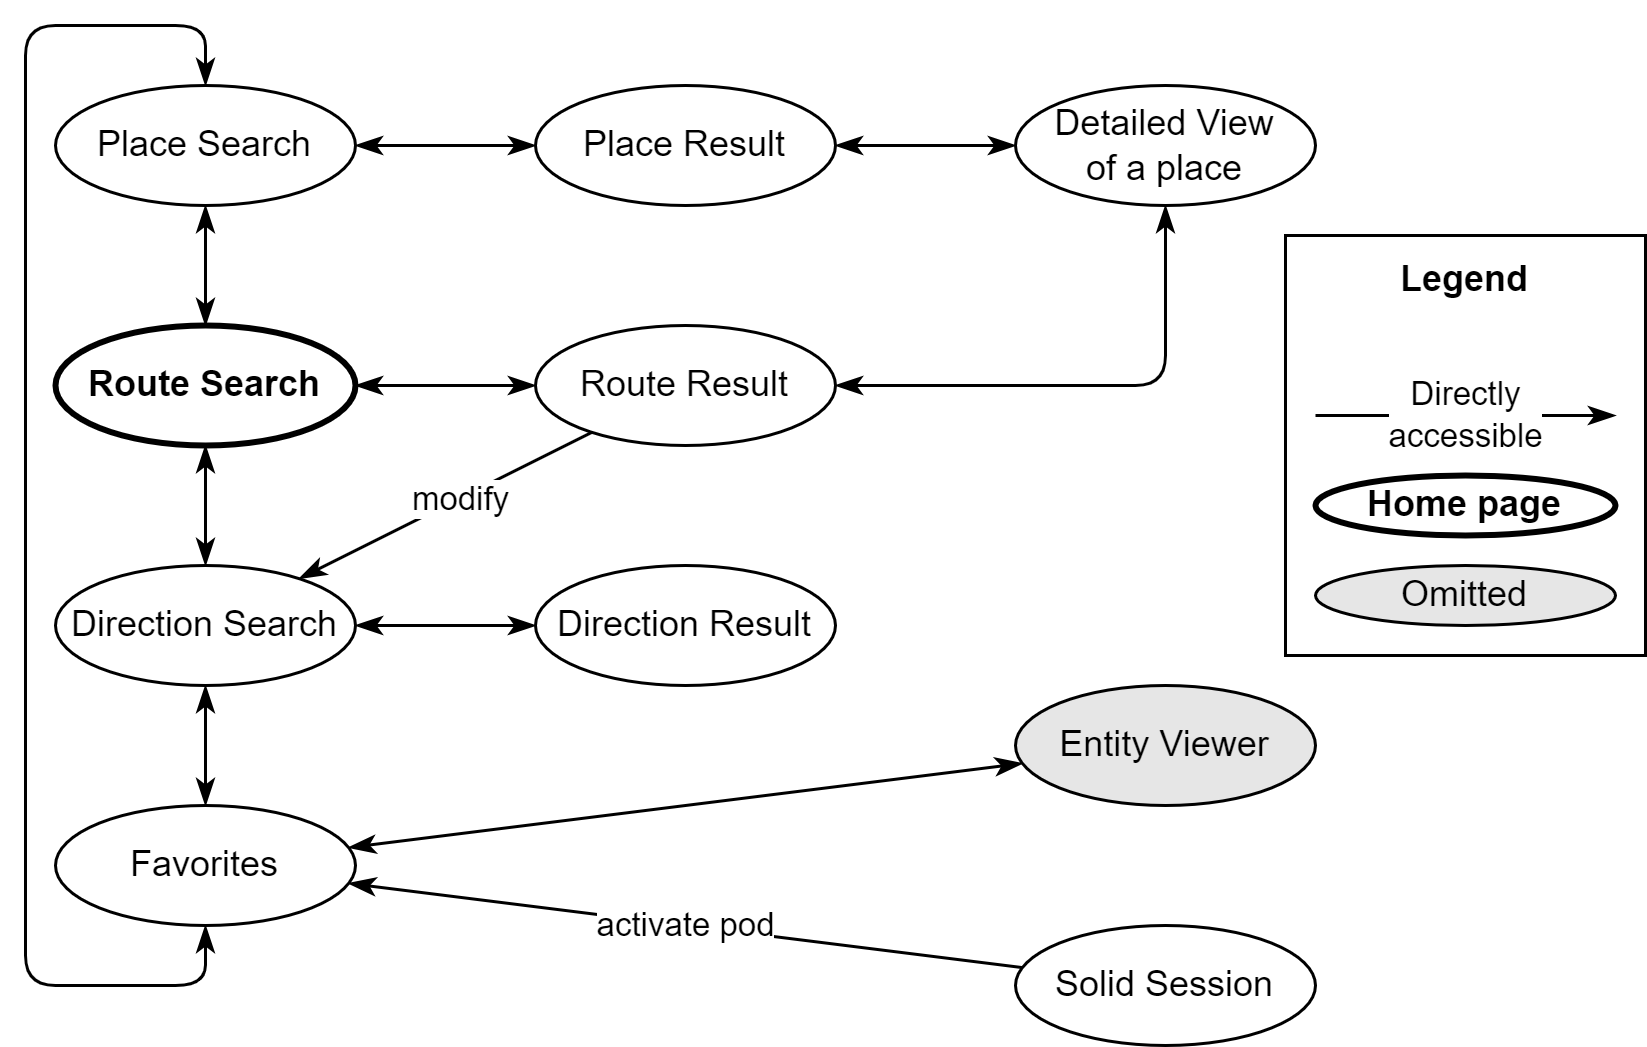
\includegraphics[width=0.9\linewidth]{img/design/ui-navigation-schema.png}
\caption{Navigation schema.}
\label{fig:ui-navigation-schema}
\end{figure}

The home page of the application is designed to carry out route searches. To fill out the request form, users need to provide a starting point, destination, arrows, and at least one category. Figures~\ref{fig:ui-dialog-select-point}, \ref{fig:ui-dialog-add-arrow}, and \ref{fig:ui-dialog-add-category} illustrate wireframe prototypes for the respective dialogs. Subsequently, the panel might reach the state shown in Figure~\ref{fig:ui-search-routes}. Please note that the starting point is yet to be defined.

After issuing a search query, the user is presented with the results, as demonstrated in Figure~\ref{fig:ui-result-routes}. Waypoint names are hyperlinked to their~re\-spec\-tive places. Additionally, users have the option to center the map on a specific waypoint and access the list of categories it belongs to by clicking the pin object within the route sequence.

Panels for searching places and directions utilize the same supporting dialogs and have only minor differences compared to route search. Their wireframes are rep\-re\-sent\-ed in Figures~\ref{fig:ui-search-places}, \ref{fig:ui-result-places}, \ref{fig:ui-search-direcs}, and \ref{fig:ui-result-direcs}.

The only thing we have not discussed regarding directions is how the system allows users to rearrange the sequence mentioned in \ref{itm:f-search-direcs-arrange}. Its points are draggable by elements consisting of six dots, and the ``Rv'' button reverses their order.

Each place in the public storage is assigned a detailed view showing all available information in a standard form, as depicted in Figure~\ref{fig:ui-detailed-view}. If present, the~exact geometry is drawn under the pin. One interesting aspect of this wireframe is that the place is already saved with a different name. The application detects the entity by its identifier and informs the user via the message box. Furthermore, the ``Save'' button is deactivated. This functionality fulfills Requirement~\ref{itm:f-entity-management-partial-copy}.

Figure~\ref{fig:ui-solid-dialog} and \ref{fig:ui-solid-panel} shed light on how to log in against a \acs{solid} server and activate an available pod. After entering an address and clicking the ``Log in'' button, the user is redirected to an external web page where they complete the~au\-then\-ti\-ca\-tion process. The appearance and actual procedure depend on the provider.

After pod activation, the user is redirected to the panel where the collection of entities is maintained. The layout of this panel view is rather straightforward; Figure~\ref{fig:ui-favorites} defines three separate sections for places, routes, and directions in the given order. All operations on entities assumed by \ref{itm:f-entity-management-favorites} are accessible via~menu buttons. The user is also informed about the type of decentralized storage used. In particular, three states are possible: device storage, \acs{solid} storage, and emergency in-memory storage as a fallback for an outdated web browser.

Up to this point, we should have gained the impression that having more than one pin drawn on the map is a common situation. All markers in the presented wireframes were drawn as circles colored with shades of grey. To enhance visual perception and improve the user experience with the application, we propose the schema listed in Table~\ref{tab:pin-colors}, which will determine pin colors in a given context.

\bgroup
\def\arraystretch{1.2}
\begin{table}[h!]
\centering\footnotesize
\begin{tabular}{ l l }
\toprule
\textbf{Pin color}
  & \textbf{Description} \\
\midrule
\textcolor{SourcePlaceColor}{$\blacksquare$ \texttt{\#2aad27}}
  & Starting point \\
\textcolor{TargetPlaceColor}{$\blacksquare$ \texttt{\#cb2b3e}}
  & Destination \\
\textcolor{CenterPlaceColor}{$\blacksquare$ \texttt{\#797979}}
  & Center point \\
\textcolor{CommonPlaceColor}{$\blacksquare$ \texttt{\#2a81cb}}
  & Not stored places \\
\textcolor{StoredPlaceColor}{$\blacksquare$ \texttt{\#9c2bcb}}
  & Stored places \\
\bottomrule
\end{tabular}
\caption{Possible colors of pins on the map and their meaning.}
\label{tab:pin-colors}
\end{table}
\egroup

The meaning of the first three rows is evident; let us concentrate on the rest. The main objective is to visually separate places in the result of a query based on whether they appear in the private storage or not. According to \ref{itm:f-entity-management-unique-places}, every point of interest in the public storage is assigned a unique identifier. Therefore, we can in\-cor\-po\-rate these identifiers into partial copies and use them while analyzing the results.

Please note that wireframes are intended for design simplification. For details on the actual user interface and its behavior, refer to Attachments~\ref{sec:documentation} and~\ref{sec:use-cases-attached}.

\clearpage

\begin{figure}
\centering
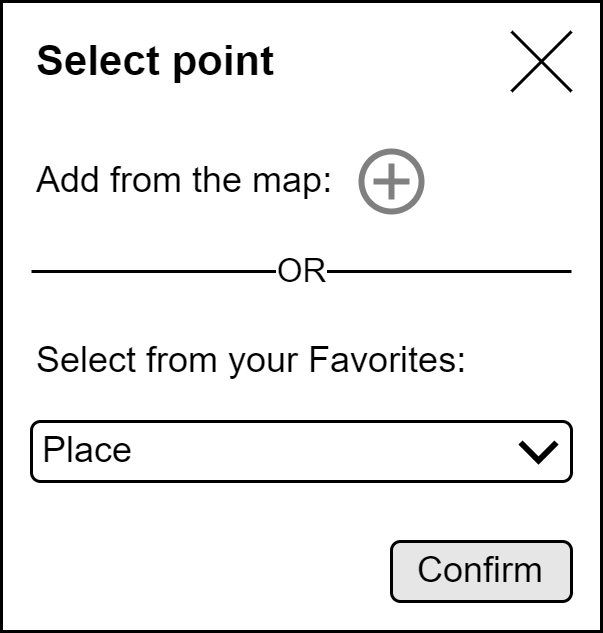
\includegraphics[width=0.45\linewidth]{img/design/ui-dialog-select-point.png}
\caption{Wireframe with the dialog for selecting a point.}
\label{fig:ui-dialog-select-point}
\end{figure}

\begin{figure}
\centering
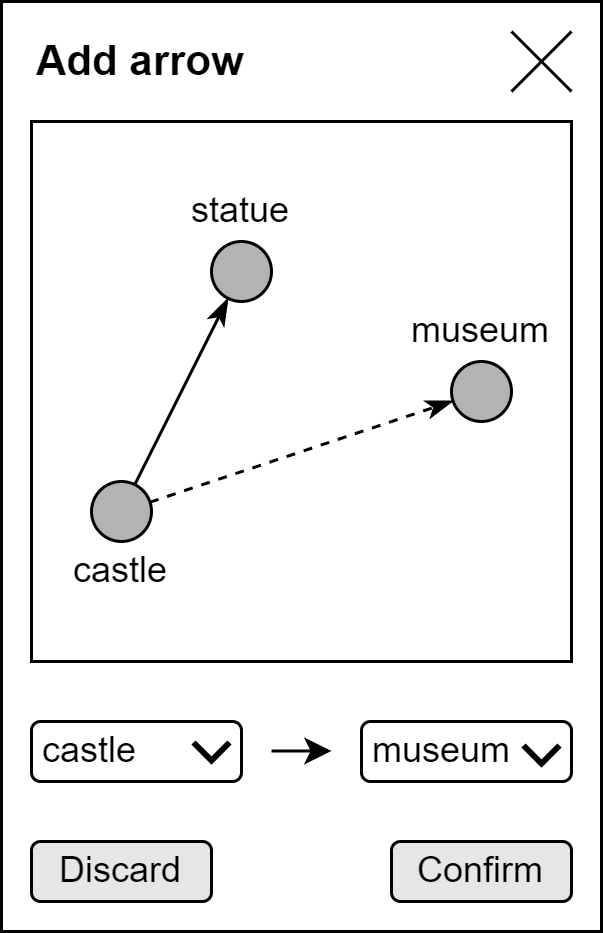
\includegraphics[width=0.45\linewidth]{img/design/ui-dialog-add-arrow.png}
\caption{Wireframe depicting the state of the dialog for con\-fig\-ur\-ing arrows. The arrow with a solid line represents a ``confirmed'' arrow, and the one with a dashed line represents a ``not confirmed'' arrow.}
\label{fig:ui-dialog-add-arrow}
\end{figure}

\clearpage

\begin{figure}
\centering
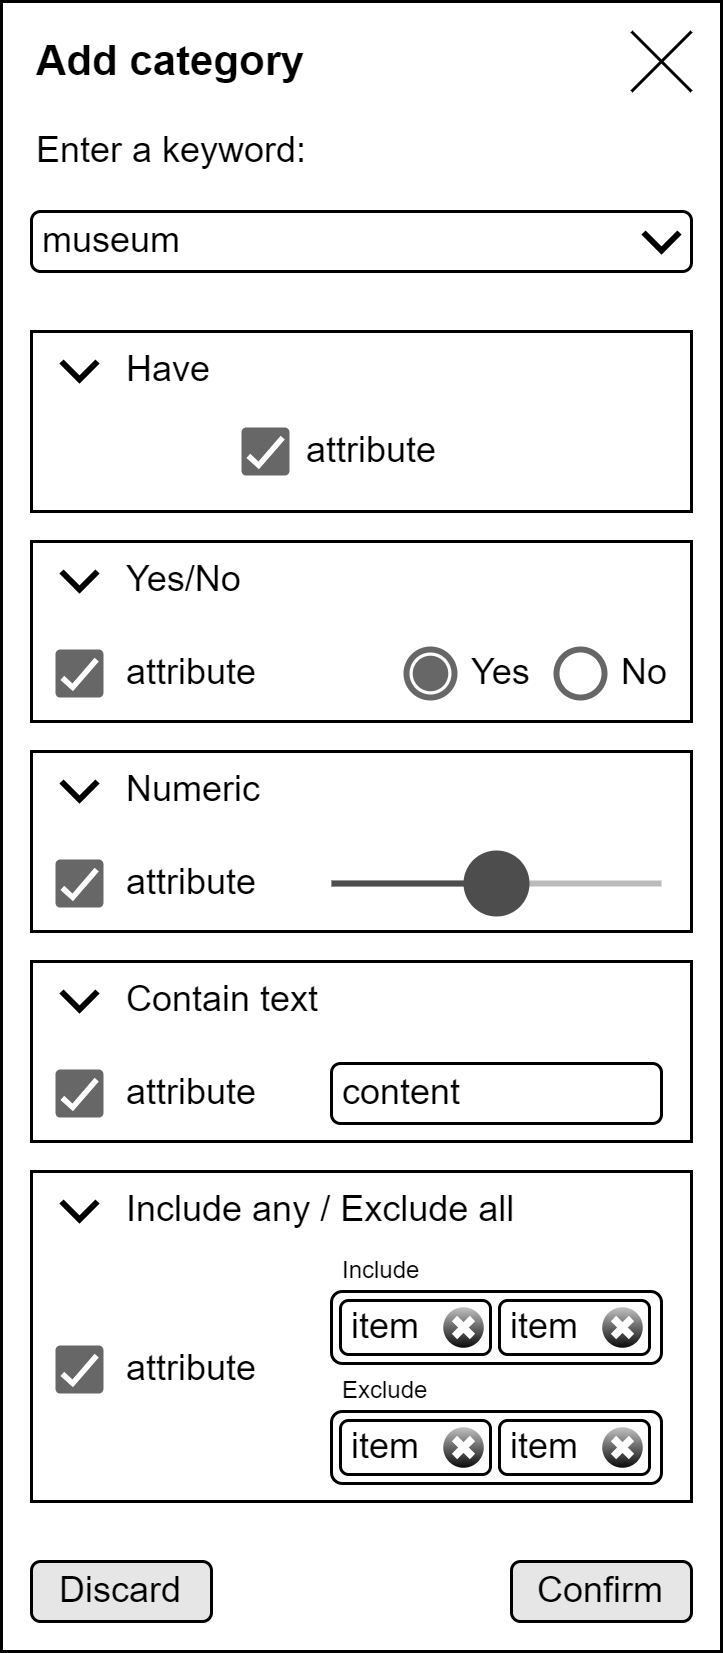
\includegraphics[width=0.55\linewidth]{img/design/ui-dialog-add-category.png}
\caption{Wireframe depicting the state of the dialog for con\-fig\-ur\-ing categories after selecting a keyword, including all five types of attribute filters.}
\label{fig:ui-dialog-add-category}
\end{figure}

\clearpage

\begin{figure}
\centering
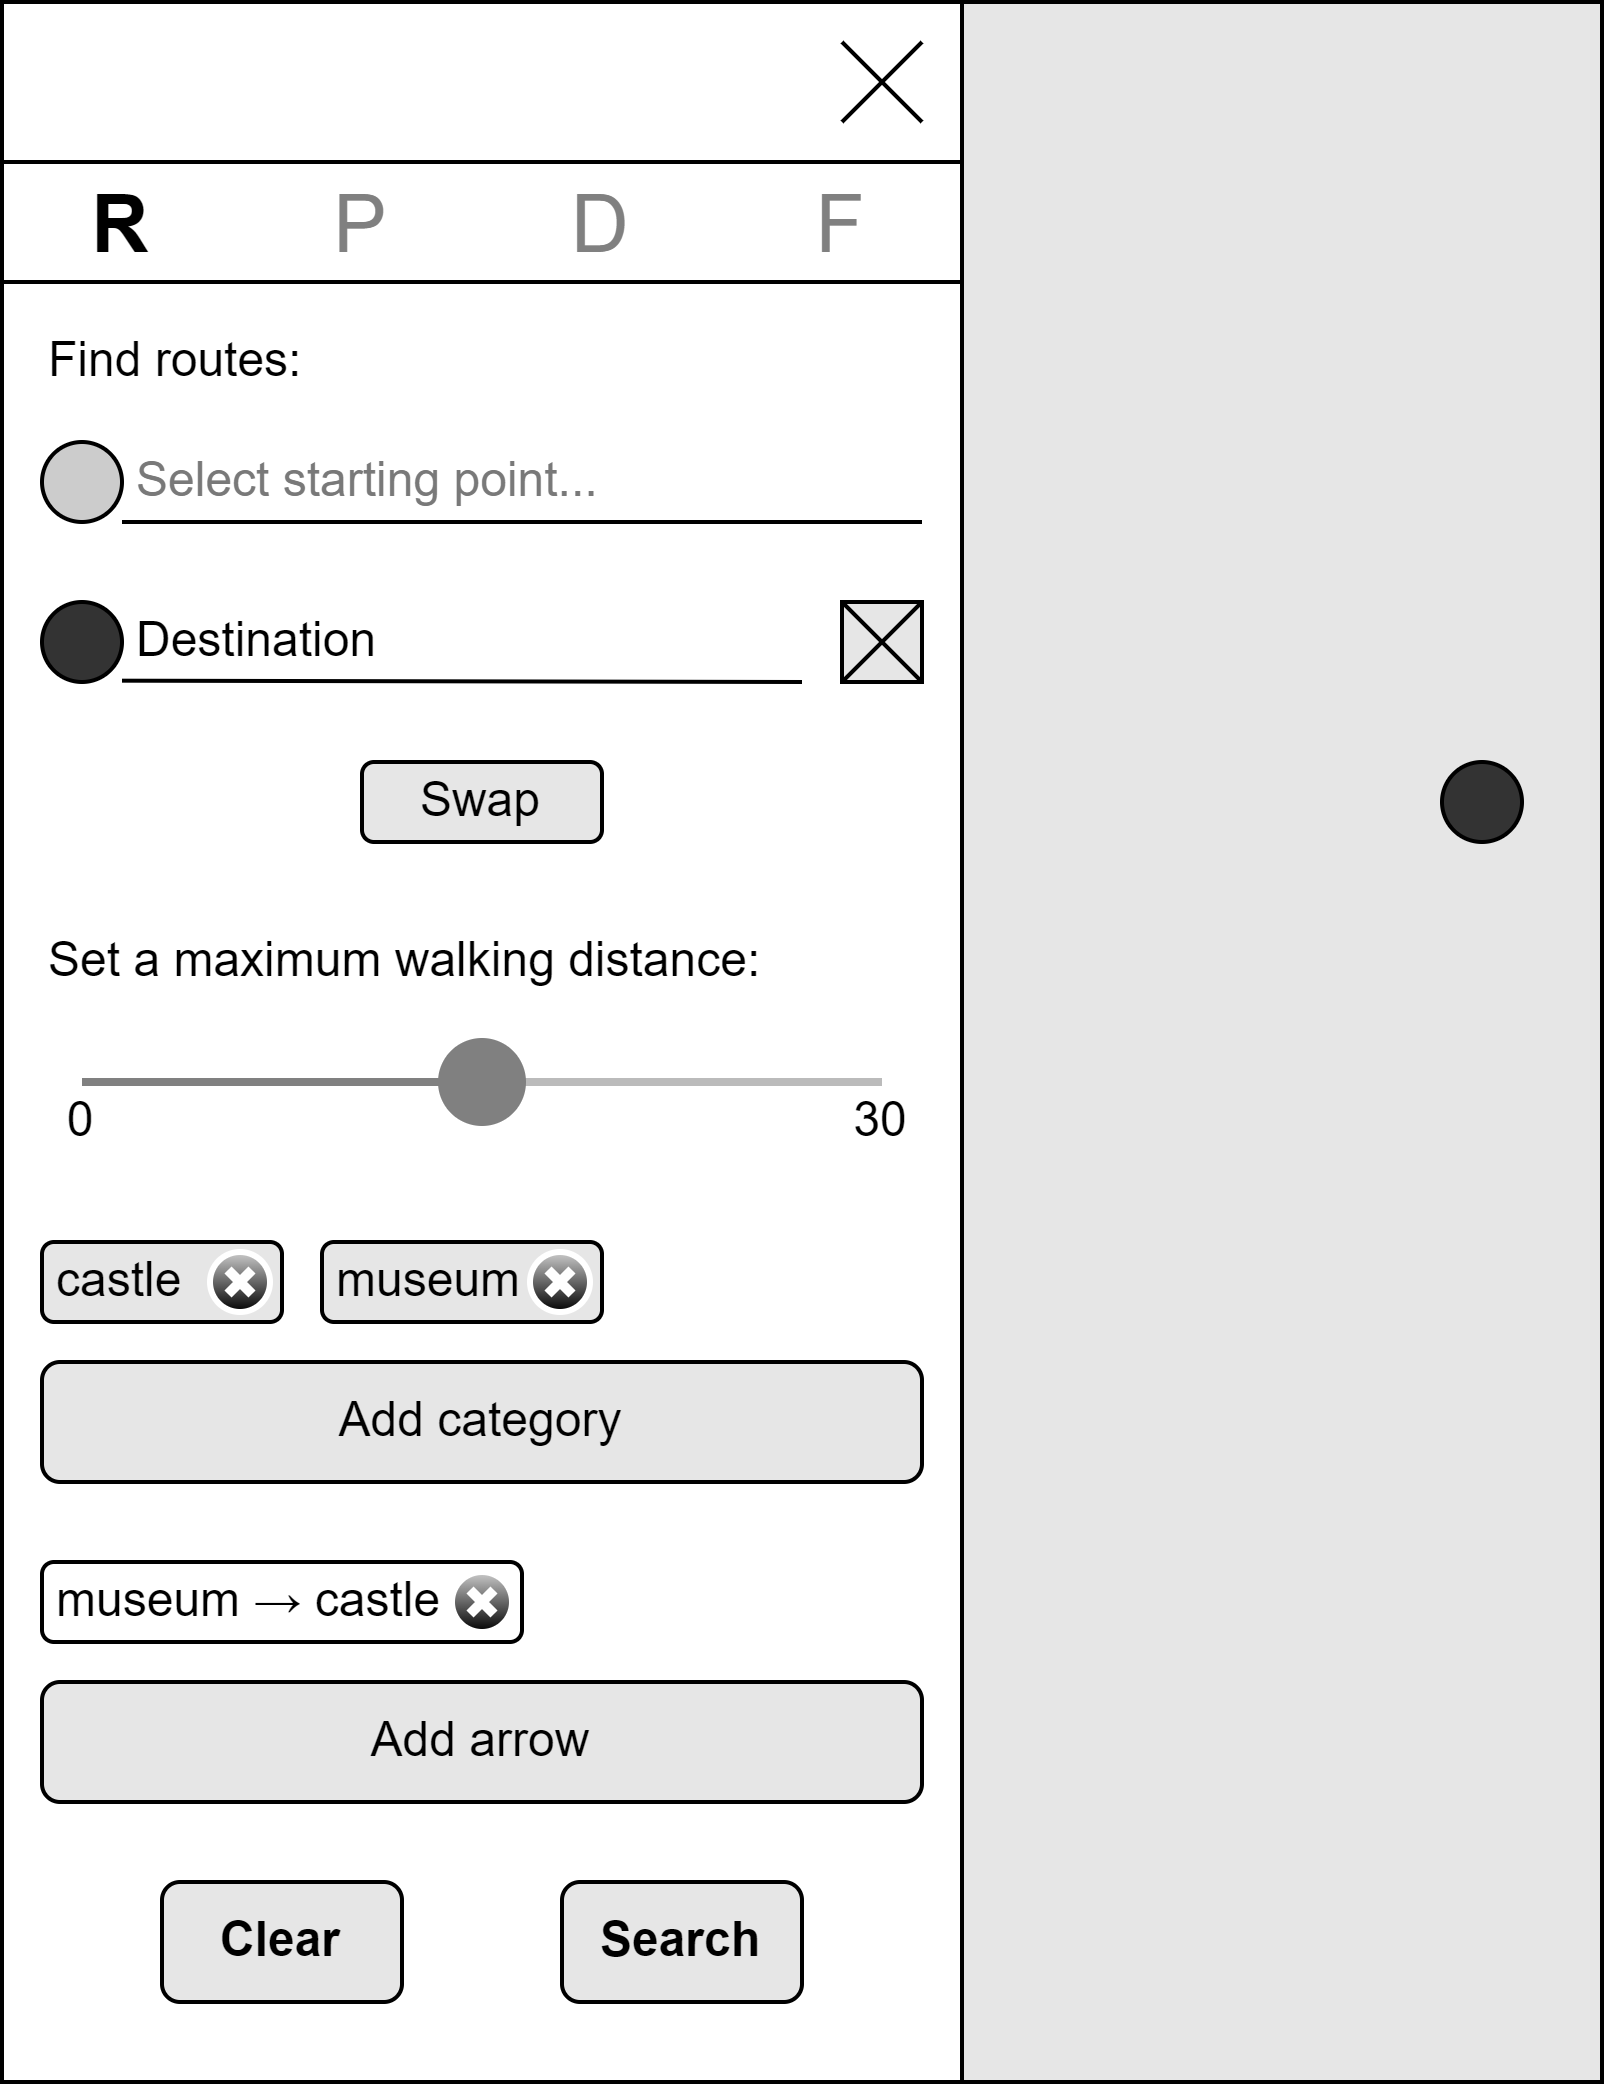
\includegraphics[width=0.67\linewidth]{img/design/ui-search-routes.png}
\caption{Wireframe with the panel for searching routes.}
\label{fig:ui-search-routes}
\end{figure}

\begin{figure}
\centering
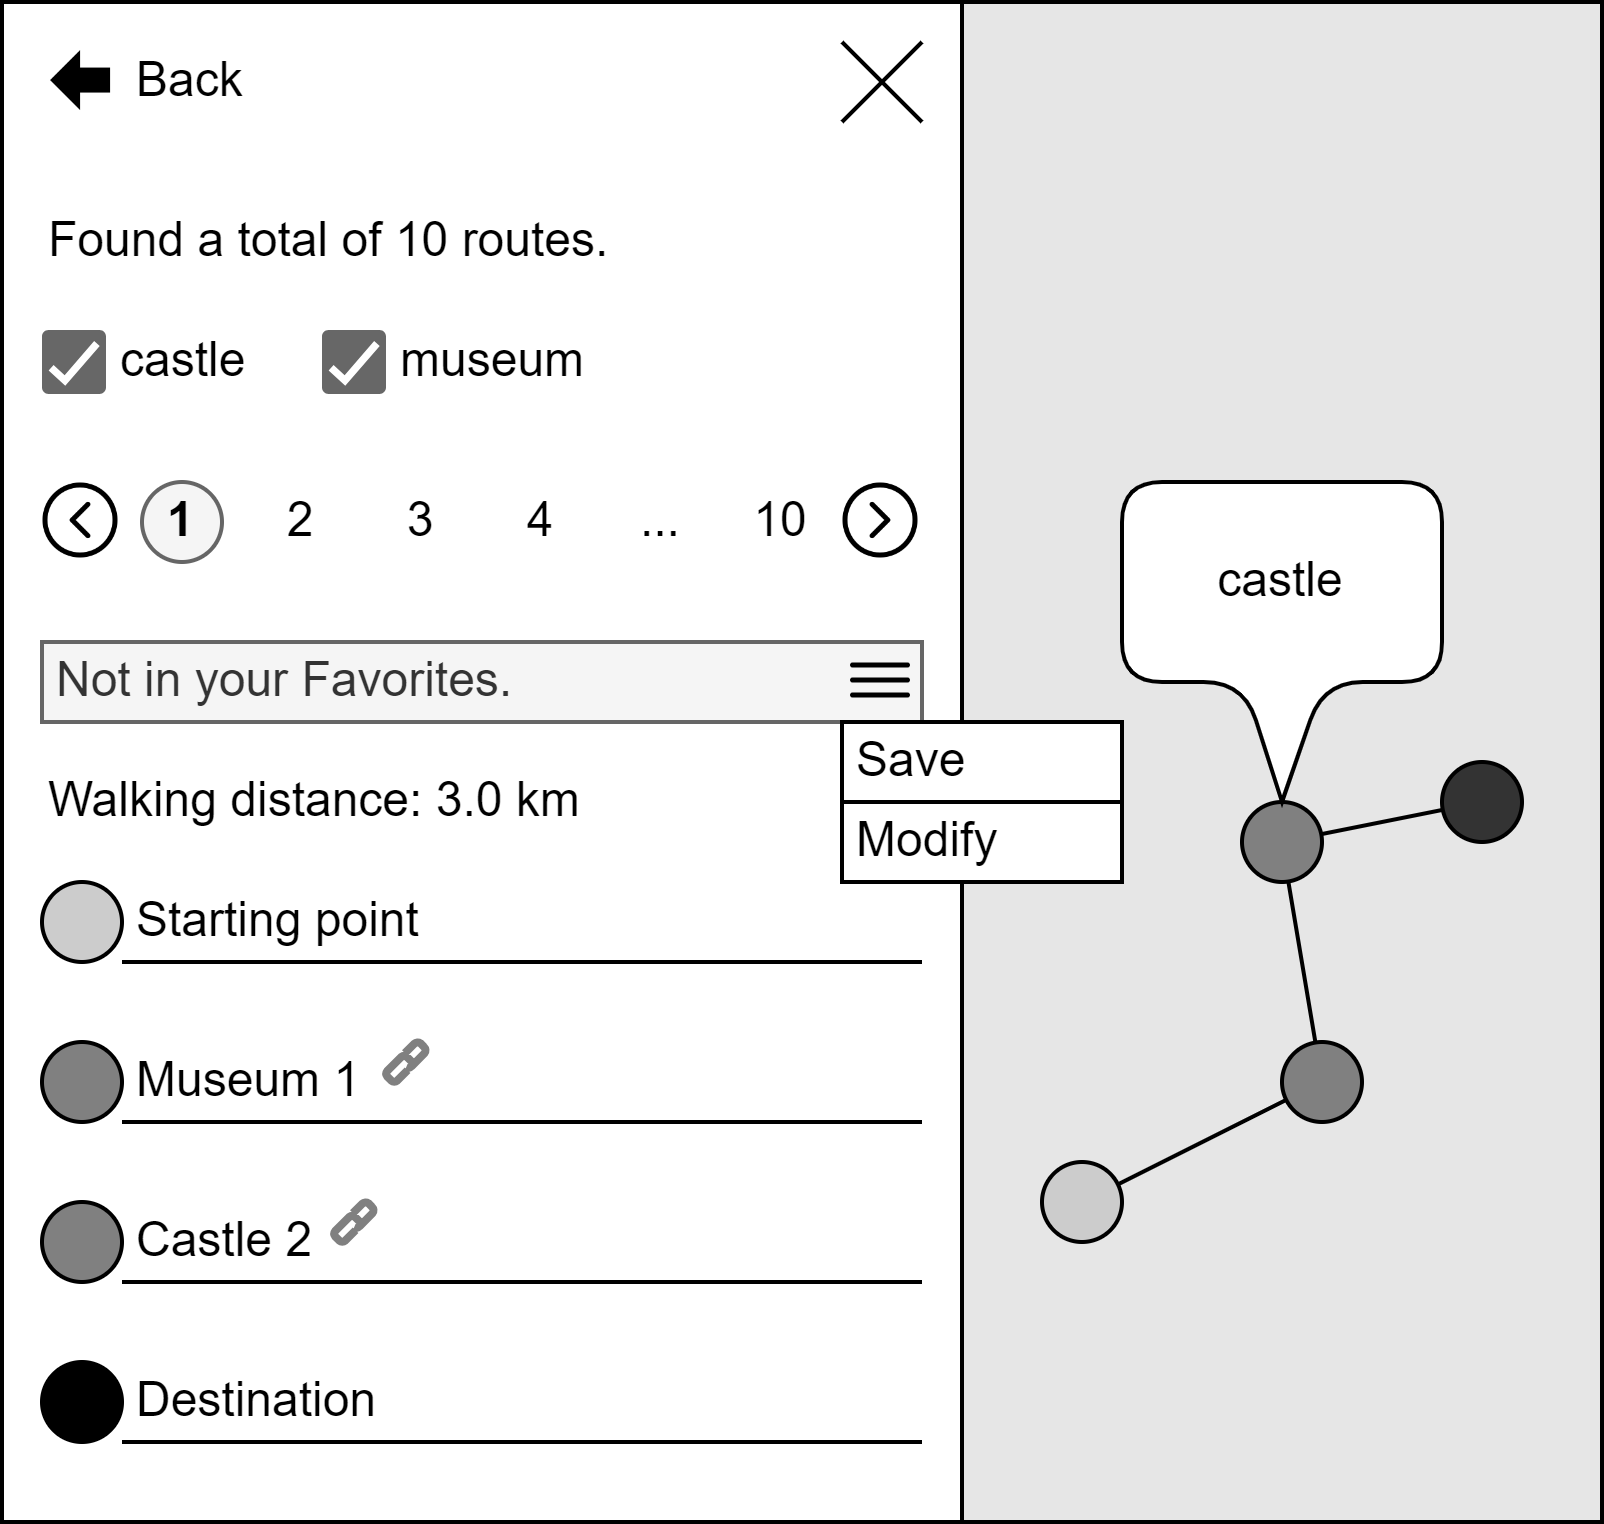
\includegraphics[width=0.67\linewidth]{img/design/ui-result-routes.png}
\caption{Wireframe with the panel showing the results of a route search.}
\label{fig:ui-result-routes}
\end{figure}

\clearpage

\begin{figure}
\centering
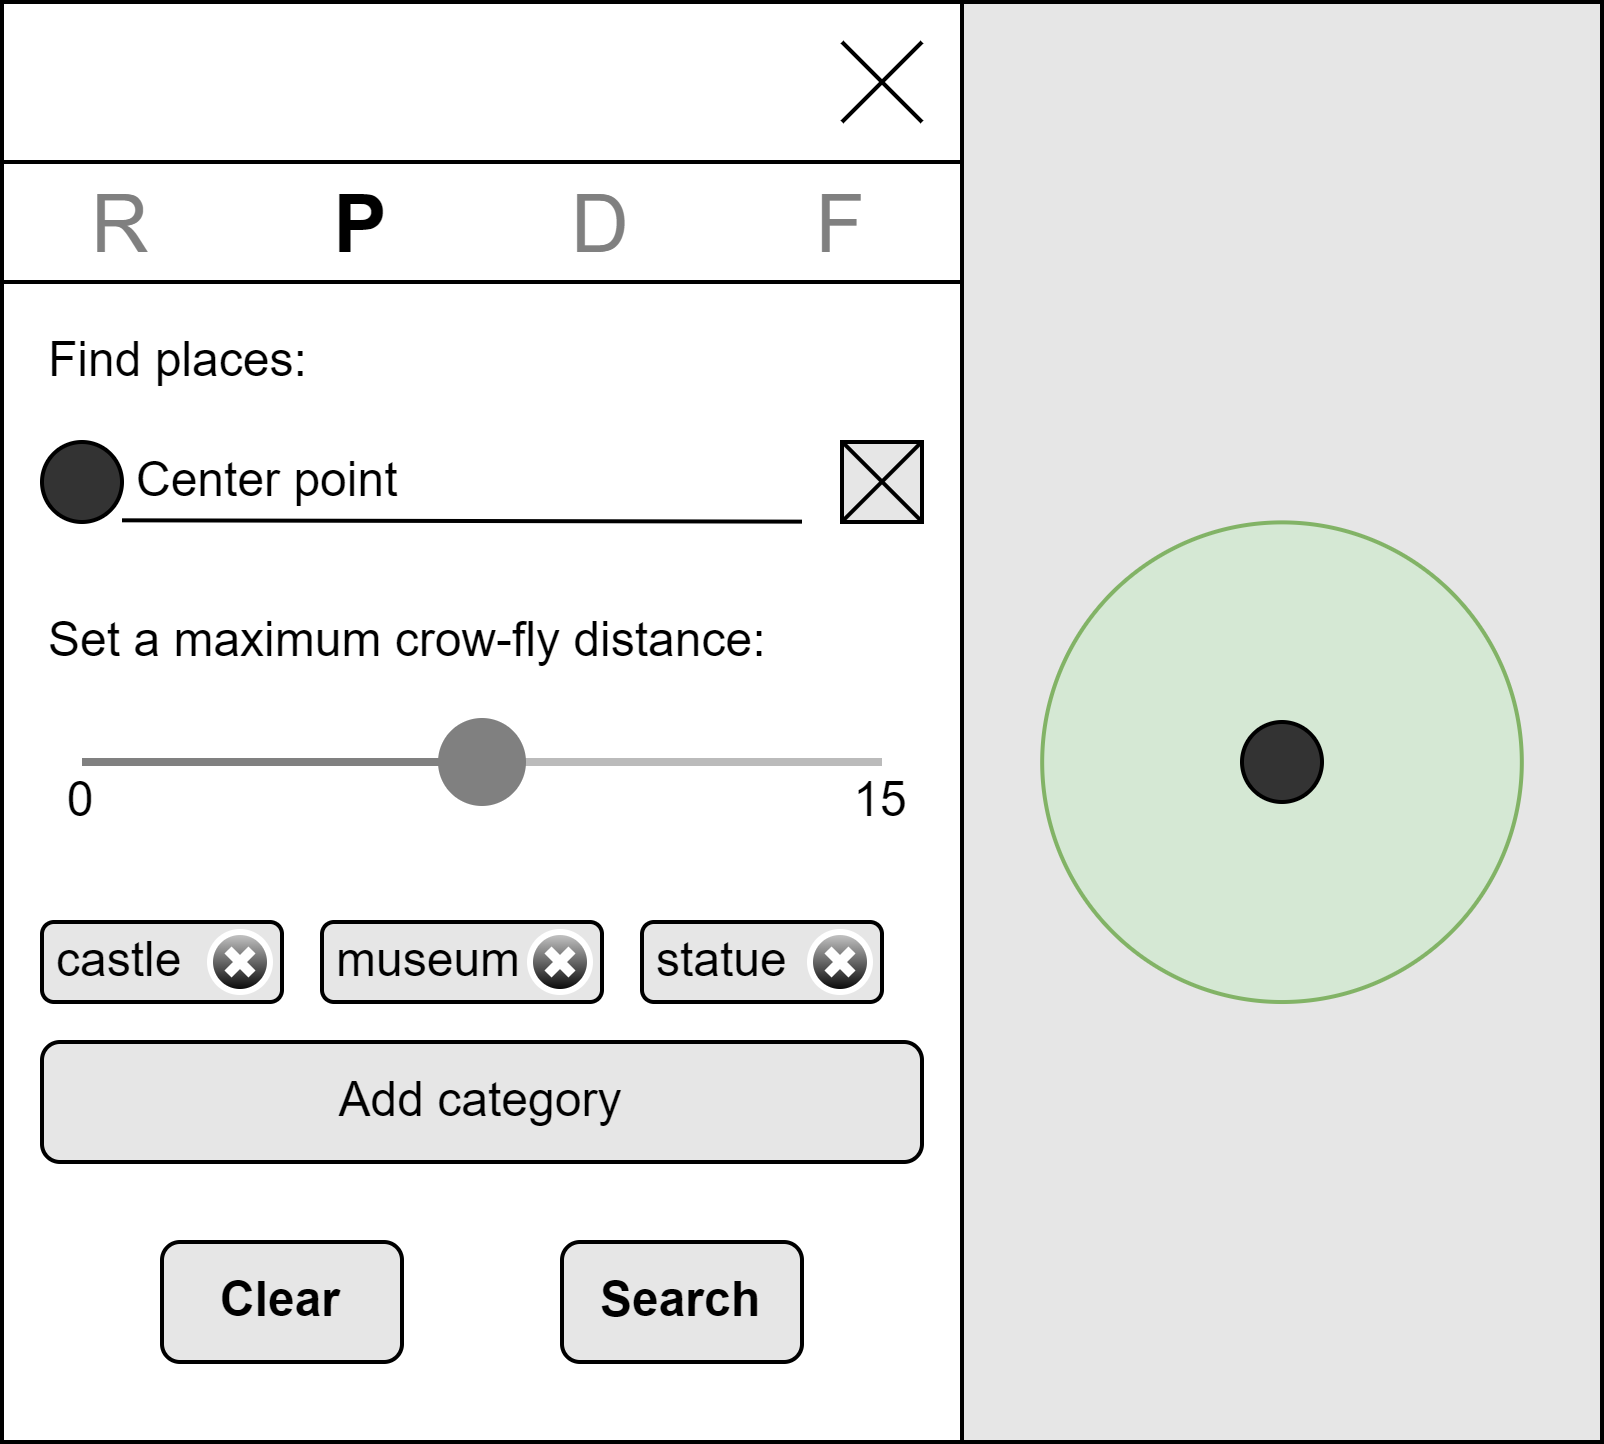
\includegraphics[width=0.67\linewidth]{img/design/ui-search-places.png}
\caption{Wireframe with the panel for searching places.}
\label{fig:ui-search-places}
\end{figure}

\begin{figure}
\centering
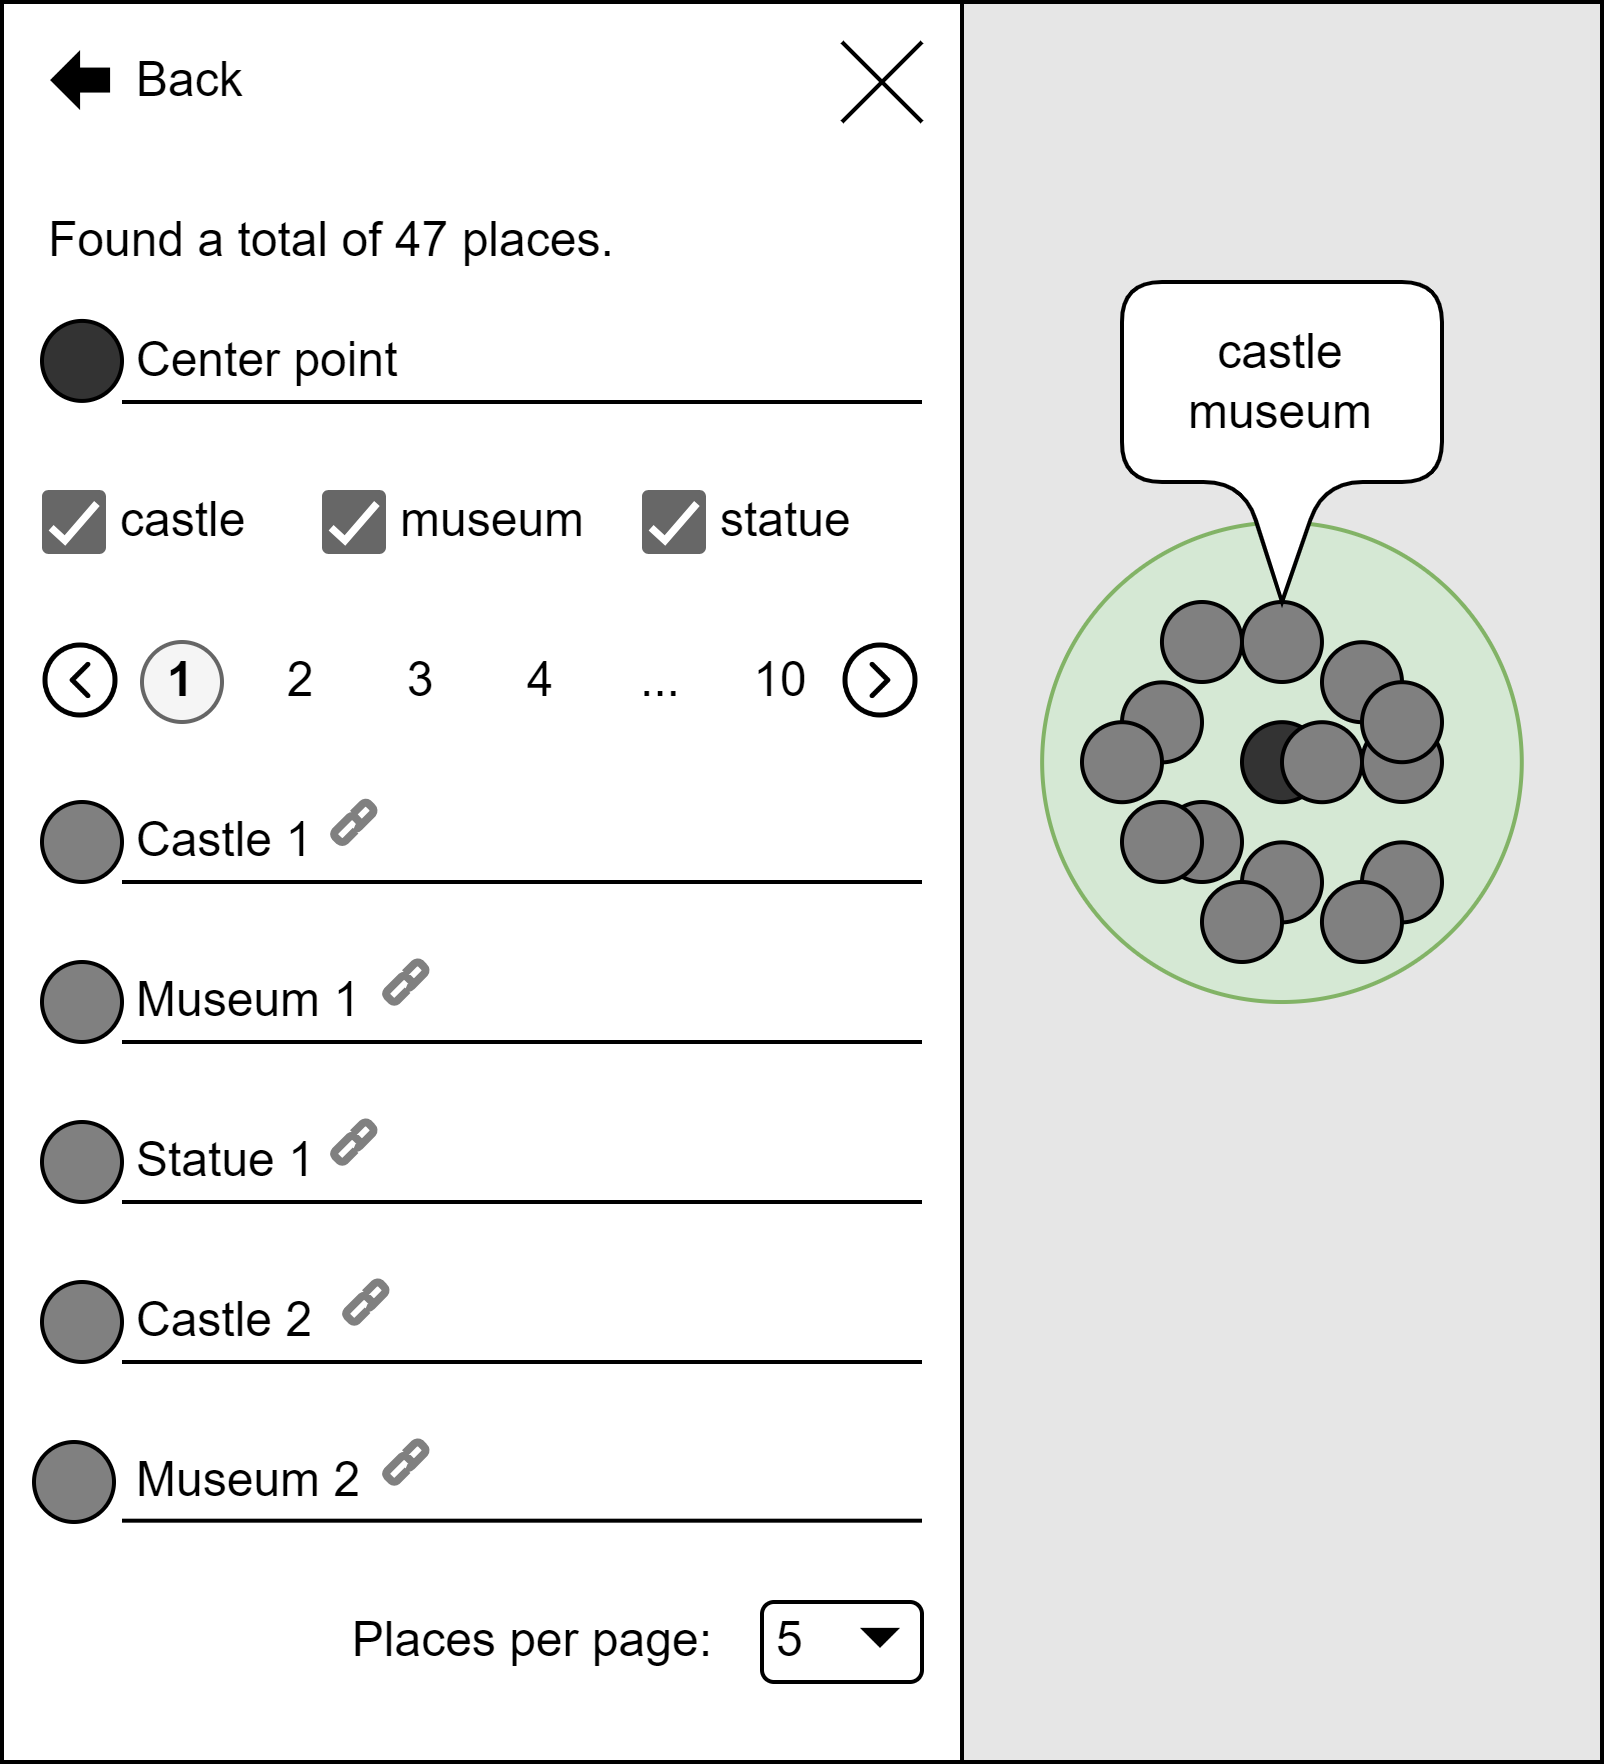
\includegraphics[width=0.67\linewidth]{img/design/ui-result-places.png}
\caption{Wireframe with the panel showing the result of a place search.}
\label{fig:ui-result-places}
\end{figure}

\clearpage

\begin{figure}
\centering
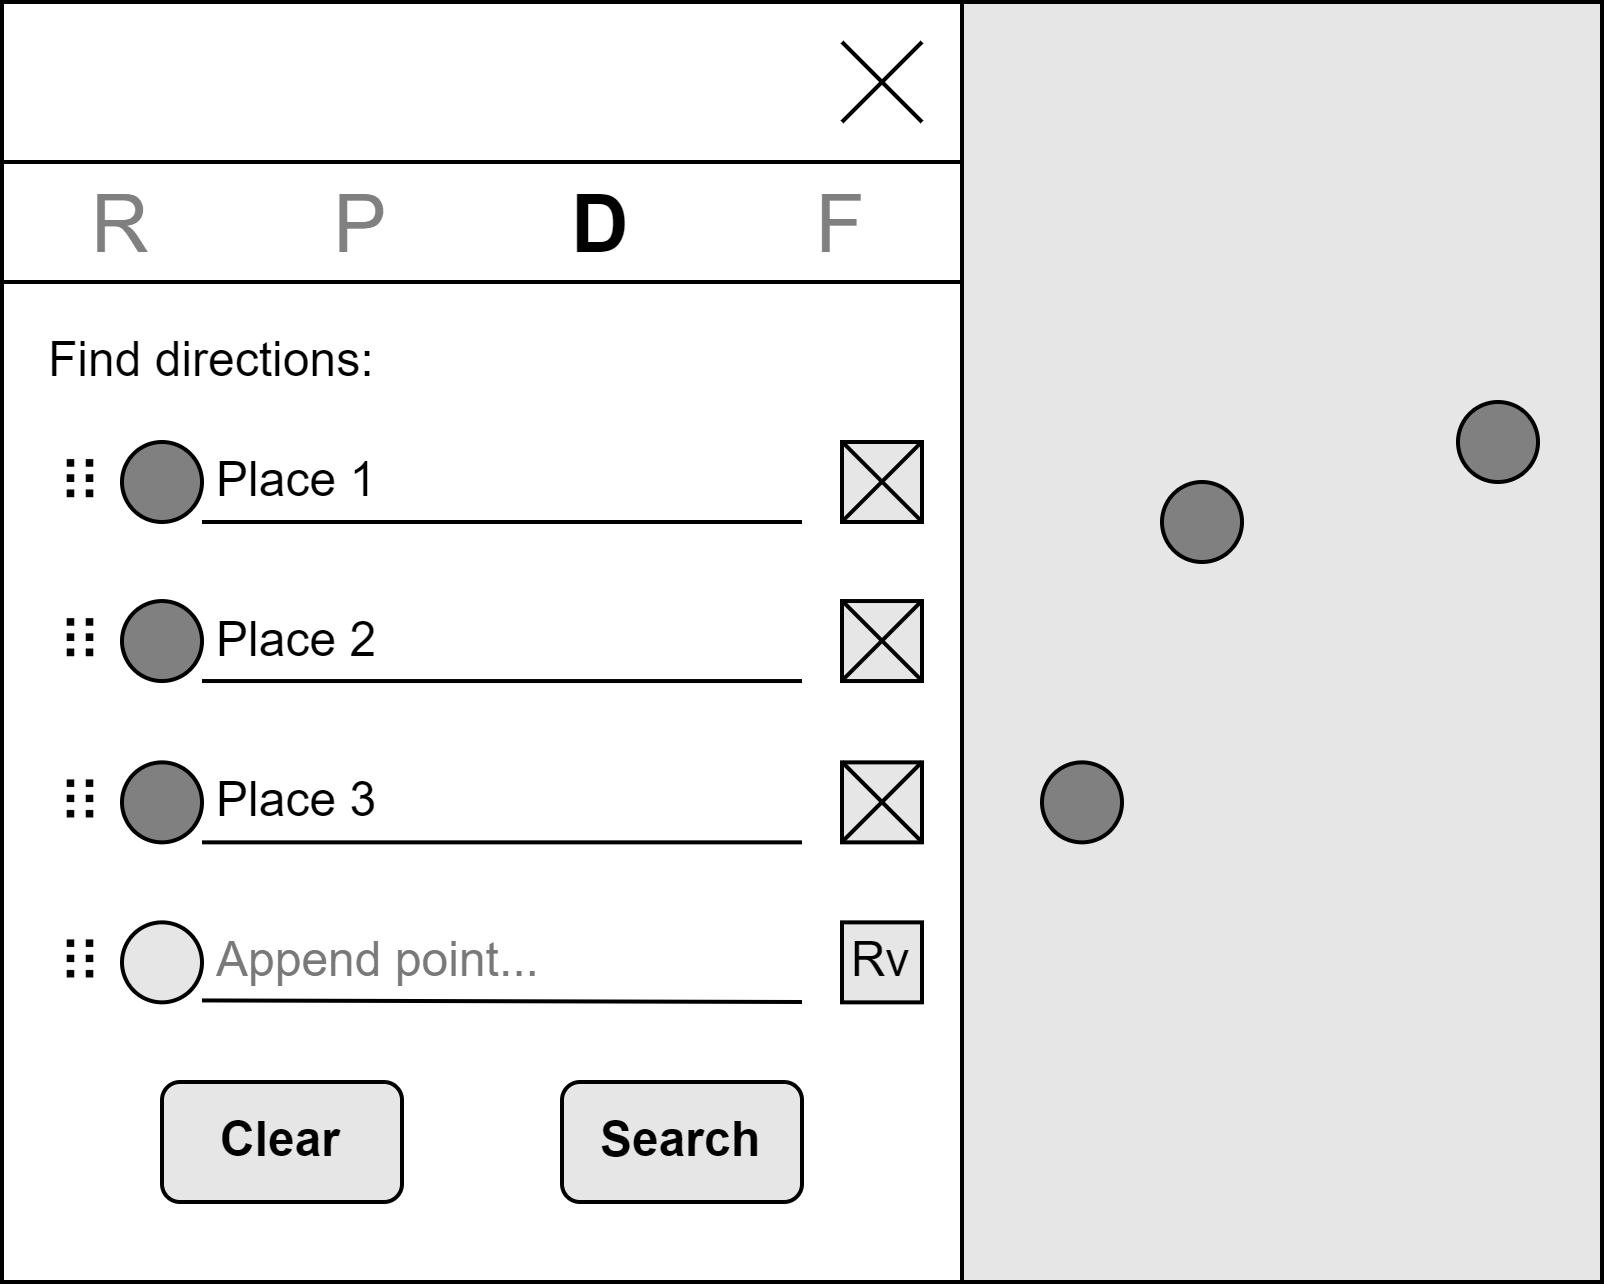
\includegraphics[width=0.67\linewidth]{img/design/ui-search-direcs.png}
\caption{Wireframe with the panel for searching directions.}
\label{fig:ui-search-direcs}
\end{figure}

\begin{figure}
\centering
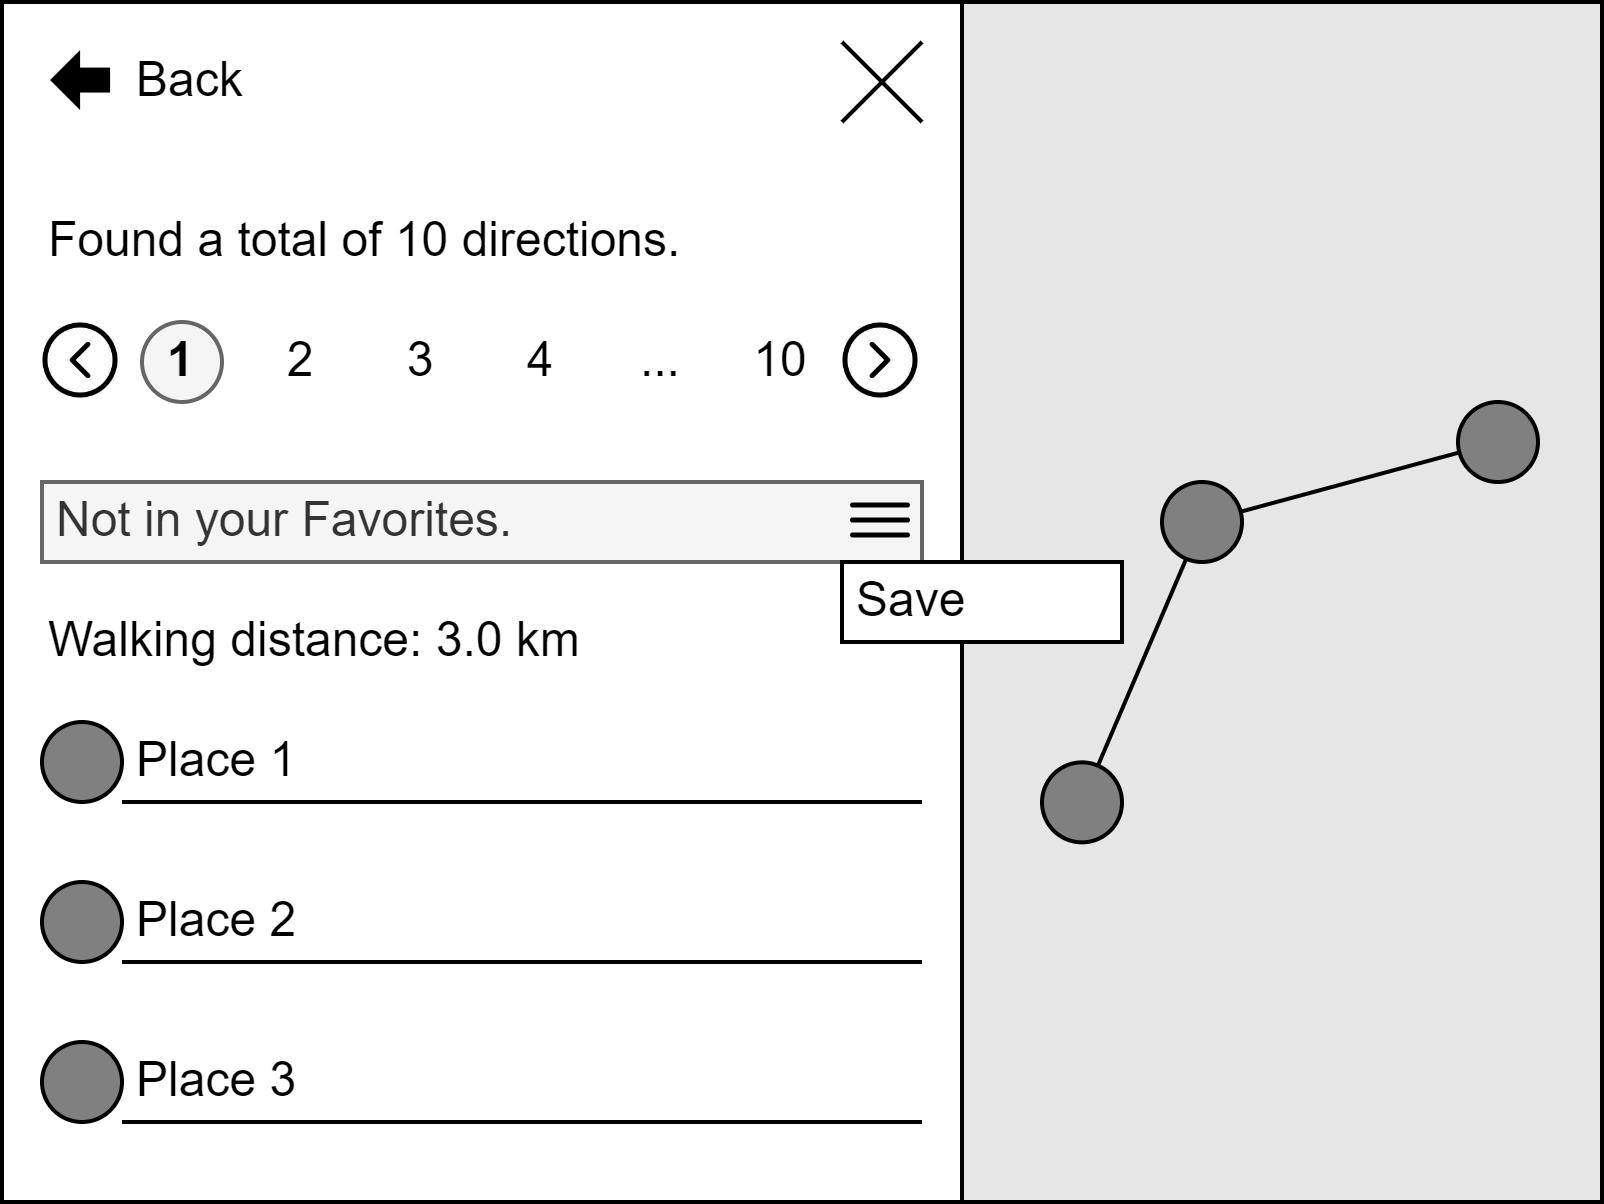
\includegraphics[width=0.67\linewidth]{img/design/ui-result-direcs.png}
\caption{Wireframe with the panel showing the results of a direction search.}
\label{fig:ui-result-direcs}
\end{figure}

\clearpage

\begin{figure}
\centering
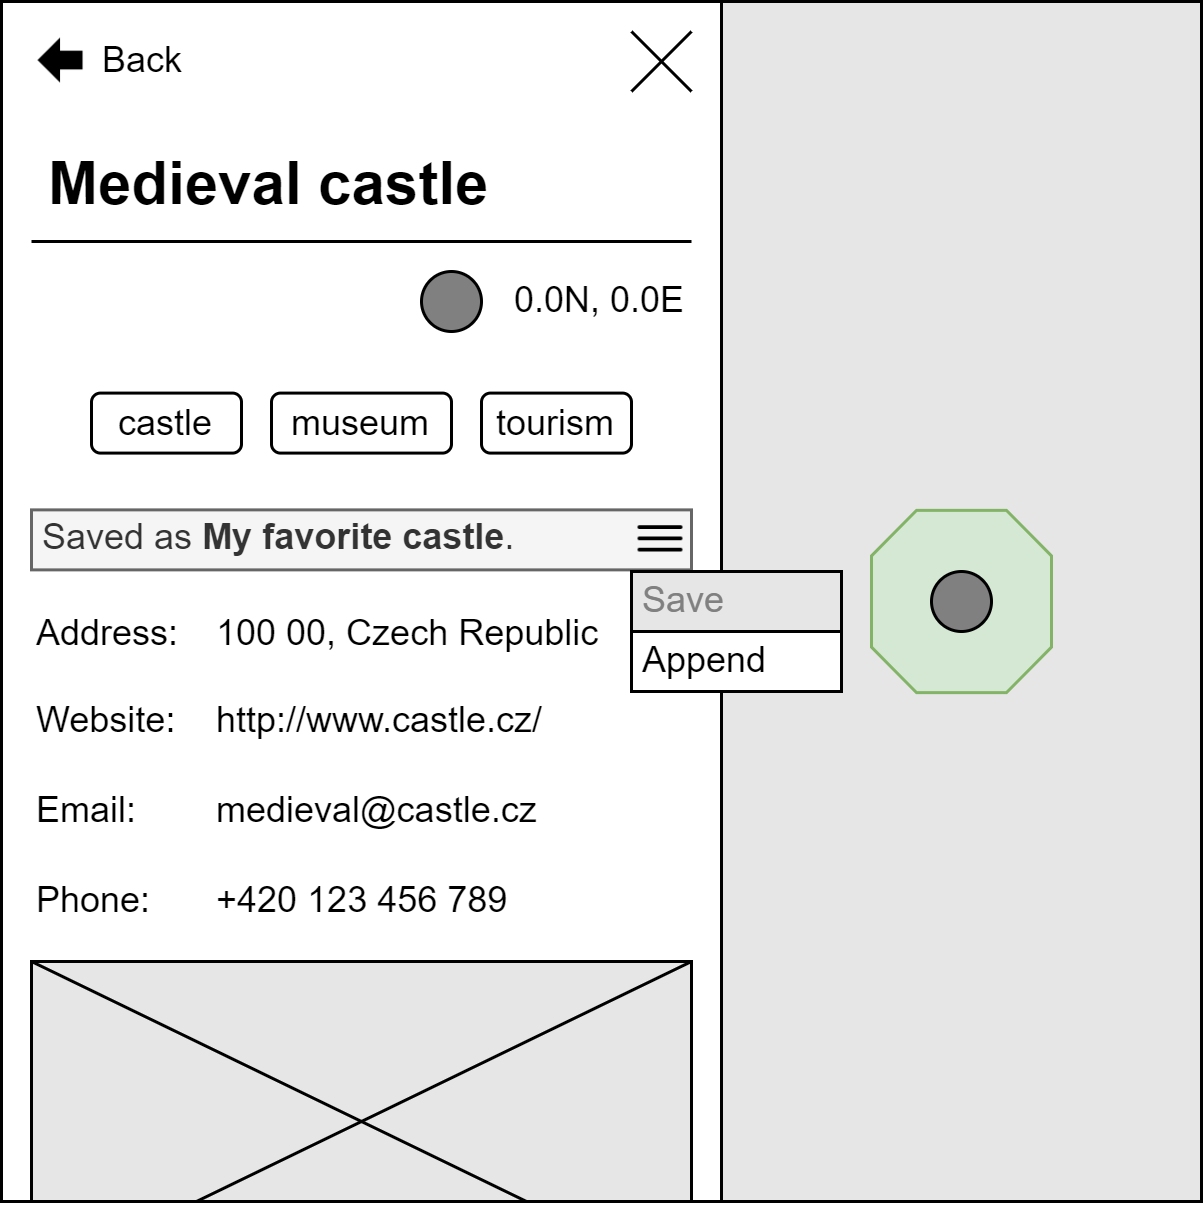
\includegraphics[width=0.68\linewidth]{img/design/ui-detailed-view.png}
\caption{Wireframe with the detailed view of a place.}
\label{fig:ui-detailed-view}
\end{figure}

\begin{figure}
  \begin{minipage}{0.48\textwidth}
    \centering
    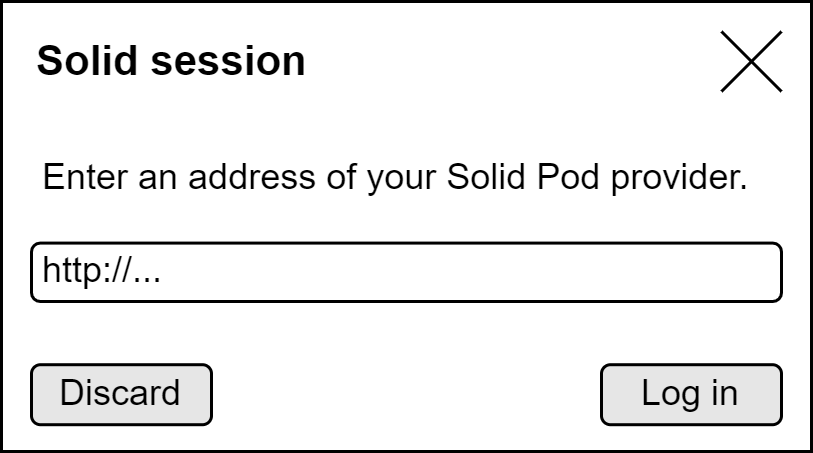
\includegraphics[width=\linewidth]{img/design/ui-solid-dialog.png}
    \caption{Wireframe with the Solid login dialog.}
    \label{fig:ui-solid-dialog}
  \end{minipage}
  \hfill
  \begin{minipage}{0.48\textwidth}
    \centering
    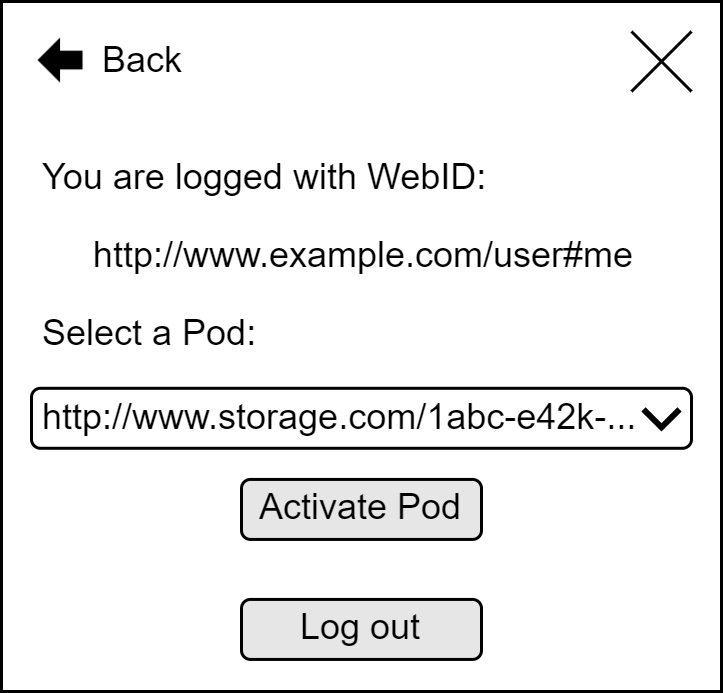
\includegraphics[width=\linewidth]{img/design/ui-solid-panel.png}
    \caption{Wireframe with the panel for activating a Solid pod.}
    \label{fig:ui-solid-panel}
  \end{minipage}
\end{figure}

\clearpage

\begin{figure}
\centering
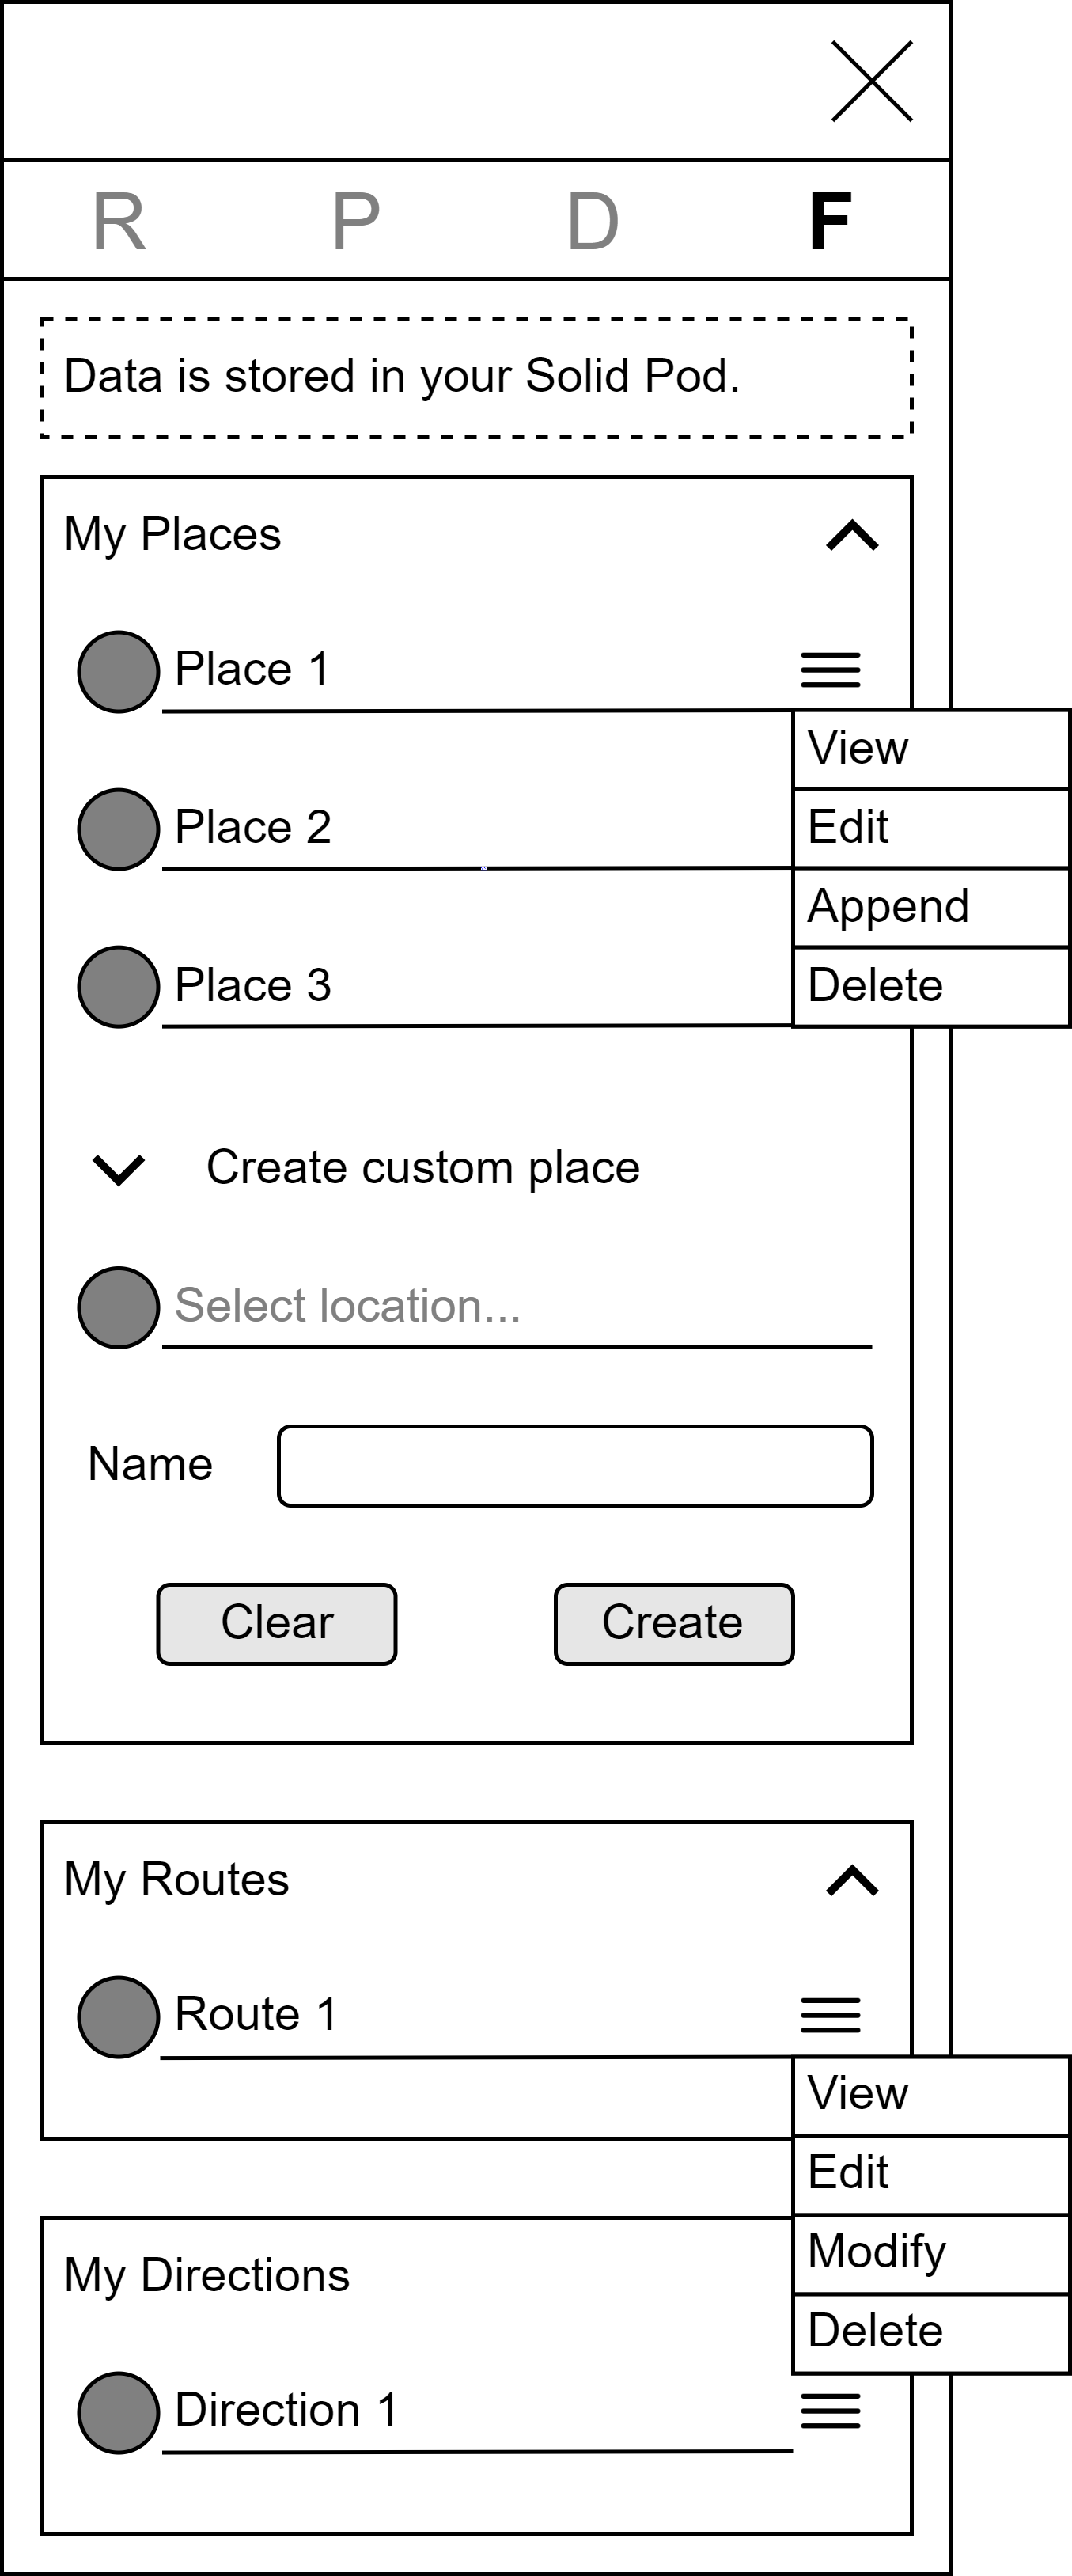
\includegraphics[width=0.55\linewidth]{img/design/ui-favorites.png}
\caption{Wireframe with the panel containing stored (favorite) entities.}
\label{fig:ui-favorites}
\end{figure}

\clearpage

\section{Architecture}\label{sec:architecture}

Solving algorithmic problems in the presence of modern web technologies requires dozens of smaller parts glued together to perform specific tasks efficiently. Their integration would be challenging without the proper level of abstraction. For this reason, the architecture of the \emph{SmartWalk} solution is demonstrated using the \emph{C4 model}~\cite{brown18}, which defines the following hierarchy of elements.

\begin{itemize}
\item A \emph{software system} brings value and makes sense to consider in isolation, as is the case with \emph{SmartWalk}.
\item A \emph{container} is a runnable part of a software system (database, mobile application that communicates over the network, web server, or even script).
\item A \emph{component} represents a non-deployable implementation of an interface used by a container.
\item \emph{Code} describes the internal organization of a component through the use of UML classes or similar notation.
\end{itemize}

Although the model defines four types of diagrams into which blocks are~gathered, we only utilize two of them --- container and component views --- as others do not provide the desired level of detail.

The architecture of our solution comprises \emph{six} essential parts, as illustrated in Figure~\ref{fig:c4-container-diagram}. It can be viewed as an implementation of the \emph{three-tier} architectural pattern with the adjustment that users store their data externally. Moreover, the \emph{backend} (or service provider) \underline{lacks} access to user data, thus addressing \ref{itm:g-decentral}.

\begin{figure}[!h]
\centering
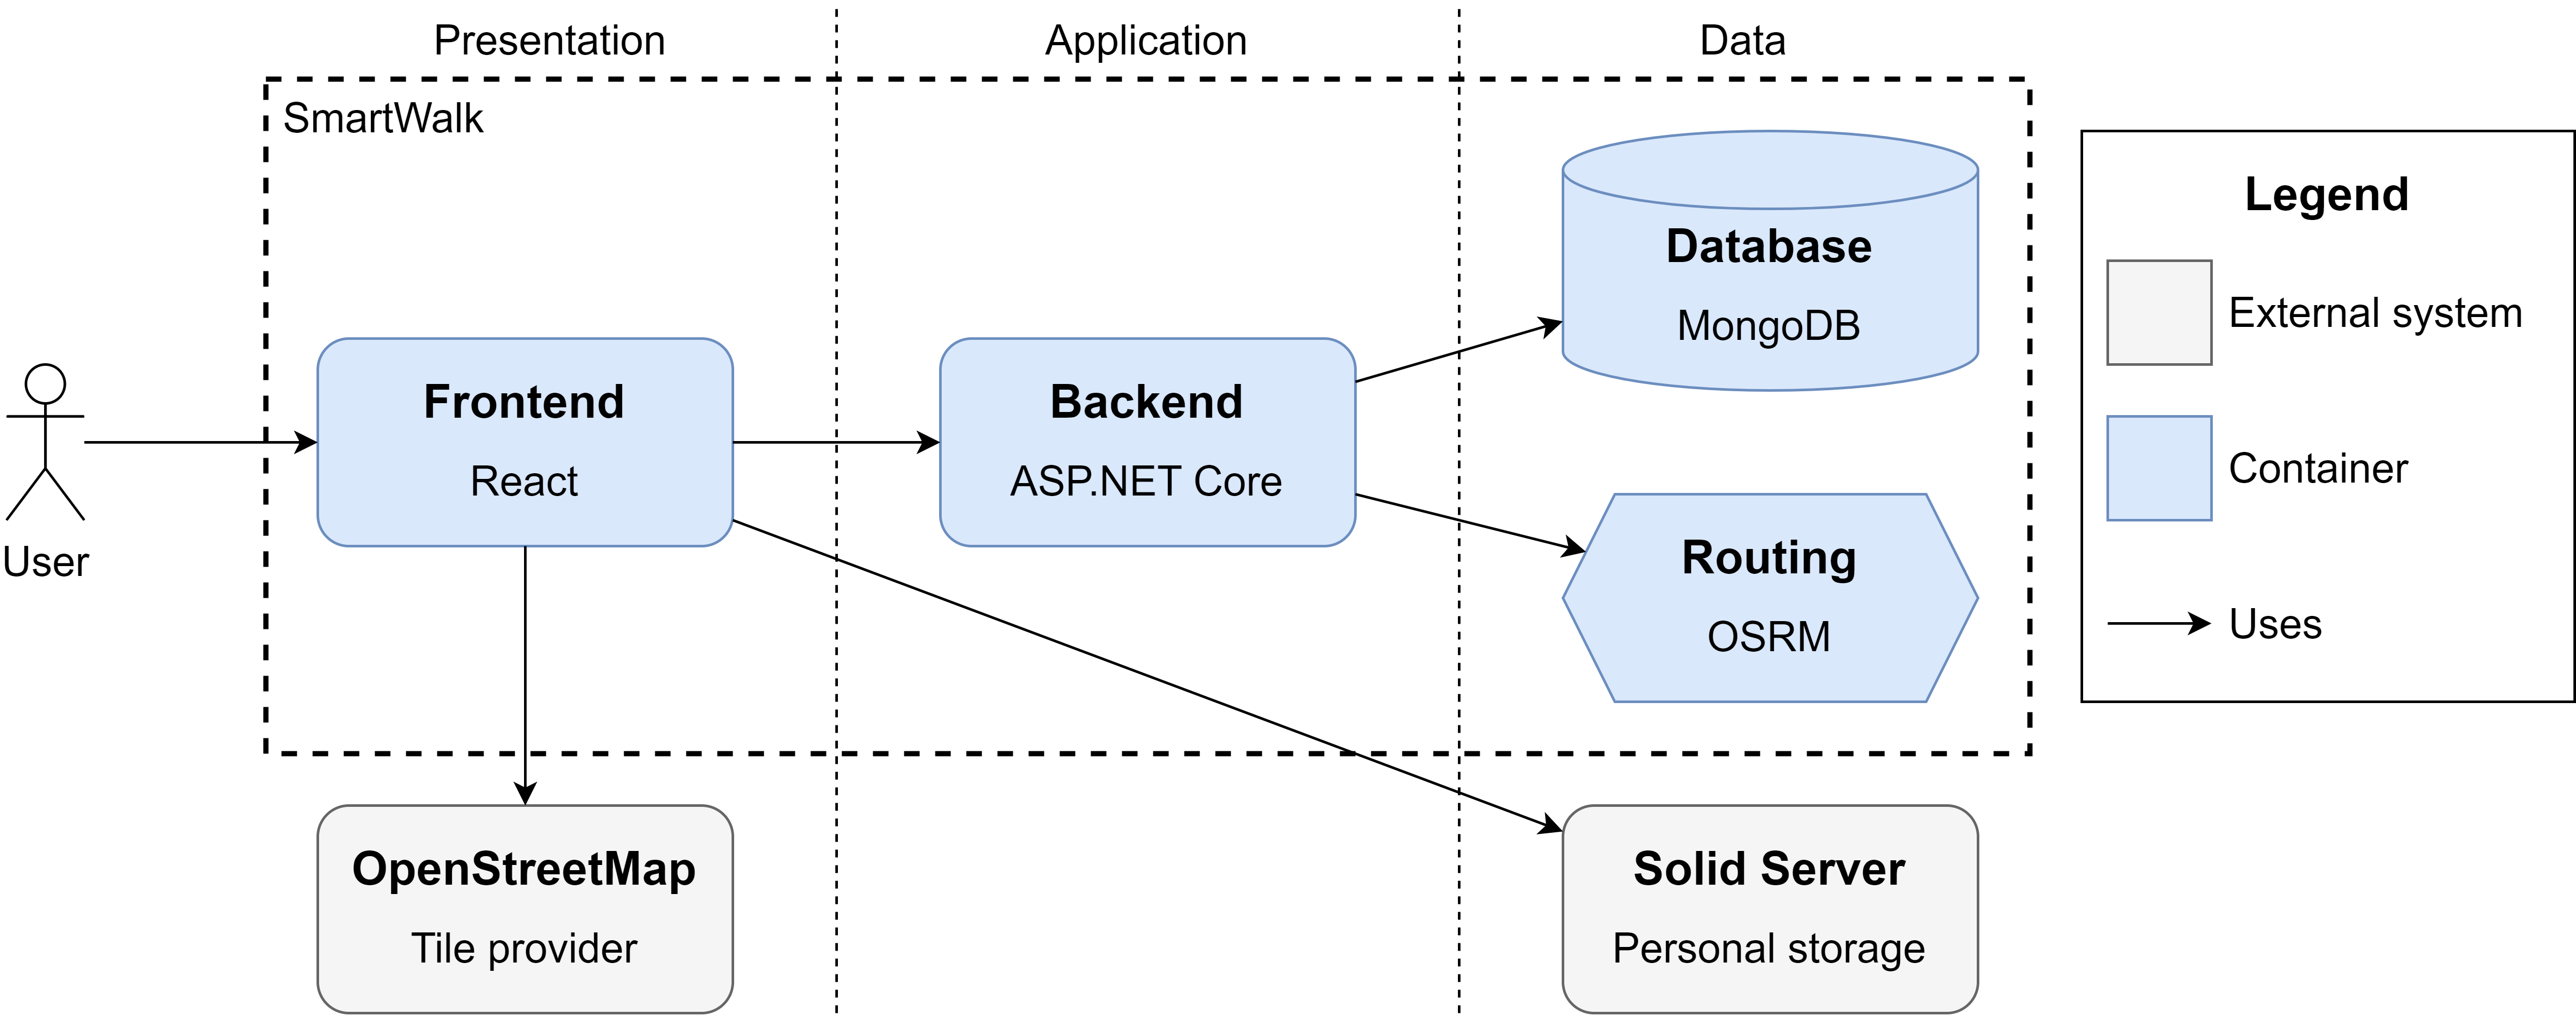
\includegraphics[width=\linewidth]{img/design/c4-container-diagram.png}
\caption{C4 container diagram of the SmartWalk software system.}
\label{fig:c4-container-diagram}
\end{figure}

The \emph{frontend} serves as an entry point to the application, offering a rich user experience. It communicates with the application tier and personal storage through a well-defined \ac{api}.

All searching and planning functionality resides within the \emph{backend}. Since~user data are stored elsewhere, we assume that only \underline{read} operations, such as generating new paths or fetching places, should be supported.

The \emph{database} and \emph{routing} are containers that supply business logic with actual data. The former acts as an entity store and search index, whereas the latter is~a specialized routing engine.

\subsection{Frontend}\label{ssec:design-frontend}

% https://martinfowler.com/articles/modularizing-react-apps.html

The \emph{frontend} is a part of the presentation tier that is exposed to a user via a web browser, providing all intended functionality. We further decompose it into five smaller components drawn in Figure~\ref{fig:c4-component-diagram-frontend}.

\texttt{PanelDrawer} mimics the user interface and navigation schema shown in Section~\ref{sec:user-interface}. \texttt{SessionProvider} ensures the login dialog and handles the proper switch over to the ``Solid Session'' panel. Other parts make possible interaction with~the environment. In particular, \texttt{Map} is responsible for loading tiles, drawing markers and vector geometries on the map. \texttt{SmartWalkAPI} provides a set of functions for retrieving data from the \emph{backend}. Finally, \texttt{Storage} is an abstraction that unifies methods for accessing both device and personal storages.

\begin{figure}[h!]
\centering
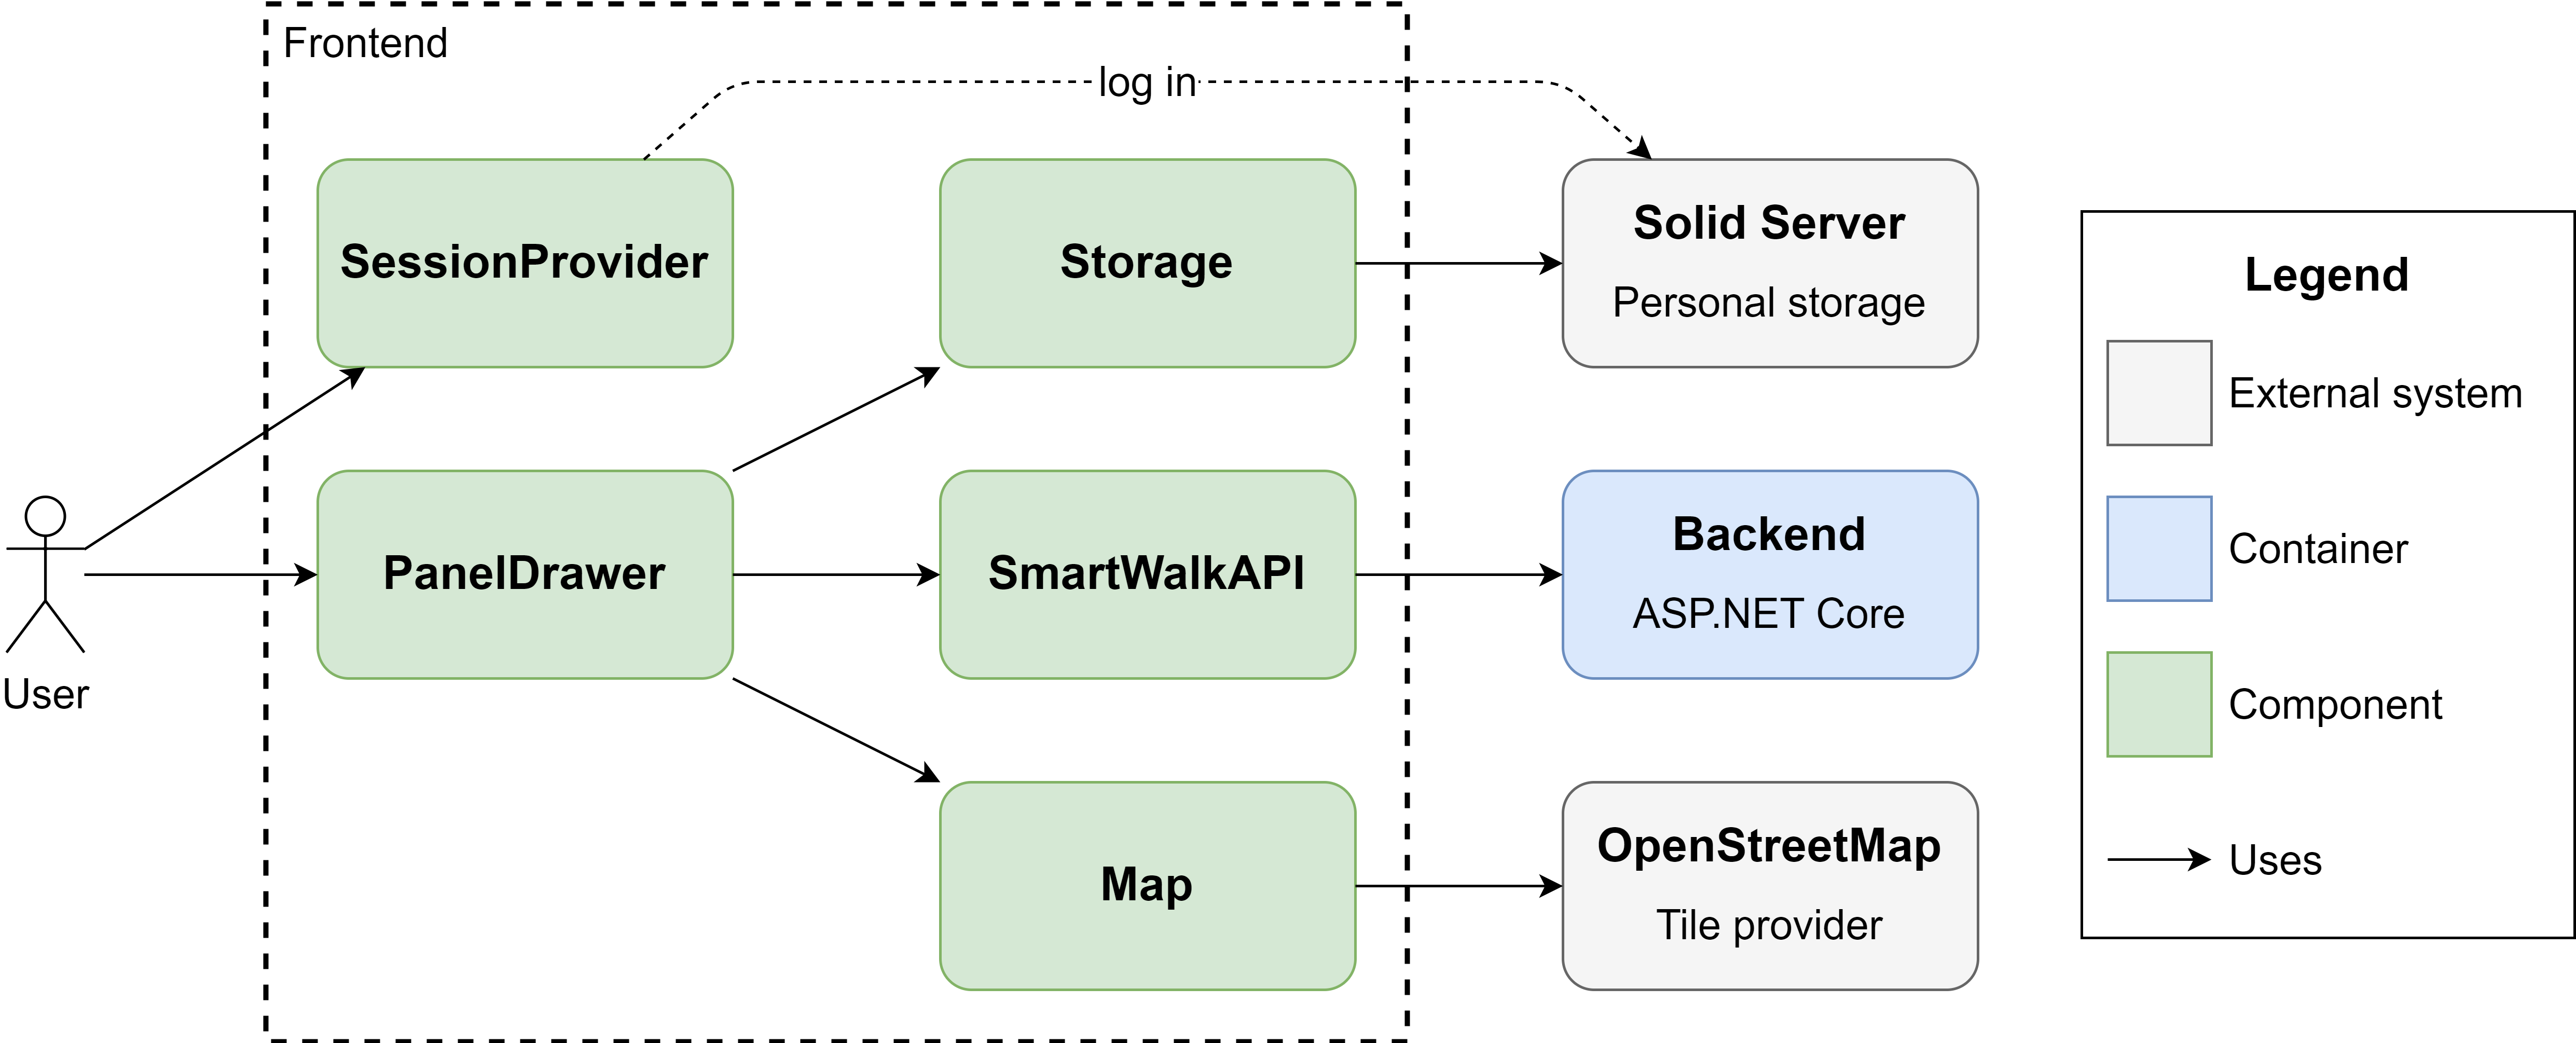
\includegraphics[width=\linewidth]{img/design/c4-component-diagram-frontend.png}
\caption{C4 component diagram of the Frontend container.}
\label{fig:c4-component-diagram-frontend}
\end{figure}

If the frontend were programmed as a classic multi-page application, navigating between pages would trigger a reload of the entire map. Hence, it is designed as a \emph{single-page application}; once loaded, the state is altered via small updates~in response to user actions, and tiles are left intact. In the remainder, we discuss~the technology stack employed in later~im\-ple\-men\-ta\-tion.

JavaScript is a natural choice for programming web solutions. However, its weak typing could make development challenging as a project grows, and catching potential errors becomes crucial. To address this issue and improve the maintainability and clarity of the codebase, we choose TypeScript\footnote{\href{https://www.typescriptlang.org/}{https://www.typescriptlang.org/}}, a statically typed JavaScript dialect with built-in type inference.

It is evident from the functional requirements that our use cases on the client side do not require extensive data processing and are limited to sending search queries and showing results. Since performance is not a top priority, the \emph{frontend} employs the React\footnote{\href{https://react.dev/}{https://react.dev/}} library. Despite not being the most efficient compared to other libraries and frameworks, it offers several advantages: a composable component-based architecture, a declarative syntax with JSX\footnote{\href{https://react.dev/learn/writing-markup-with-jsx}{https://react.dev/learn/writing-markup-with-jsx}} extension similar to HTML markup, and an intuitive unidirectional data flow where changes are propagated from parents to their nested components.

\subsection{Backend}\label{ssec:design-backend}

% https://refactoring.guru/
% https://aspiringcraftsman.com/2007/08/25/interactive-application-architecture/

The next container, the \emph{backend}, is related to the application tier. Its internal structure, revealed in Figure~\ref{fig:c4-component-diagram-backend}, loosely follows the \ac{adr} pattern~\cite{adr}. \acs{adr} is an alternative to the classic Model View Controller (MVC), offering better abstractions for \acs{http}-based services with distinct client and server sides.

\texttt{TController} receives a request object and performs validation or parsing to reject malformed input early, similar to the \texttt{Action} in \acs{adr}. Well-formed data is then handed over to the corresponding domain-level \texttt{THandler}, a re\-al\-iza\-tion of a targeted use case. \texttt{TResponder} is responsible for completing the response object based on three possible outcomes: a valid result of a calculation, an internal~server error, or failed validation. Finally, \texttt{Gateways} are entities of the data access layer that implement abstract interfaces.

Please note the letter \texttt{T} in the names of some elements, indicating the generic nature of the diagram. A total of \emph{five} distinct pipelines are implemented following the same concepts. The actual routing and invocation of the proper controller are details delegated to the framework.

\begin{figure}[h!]
\centering
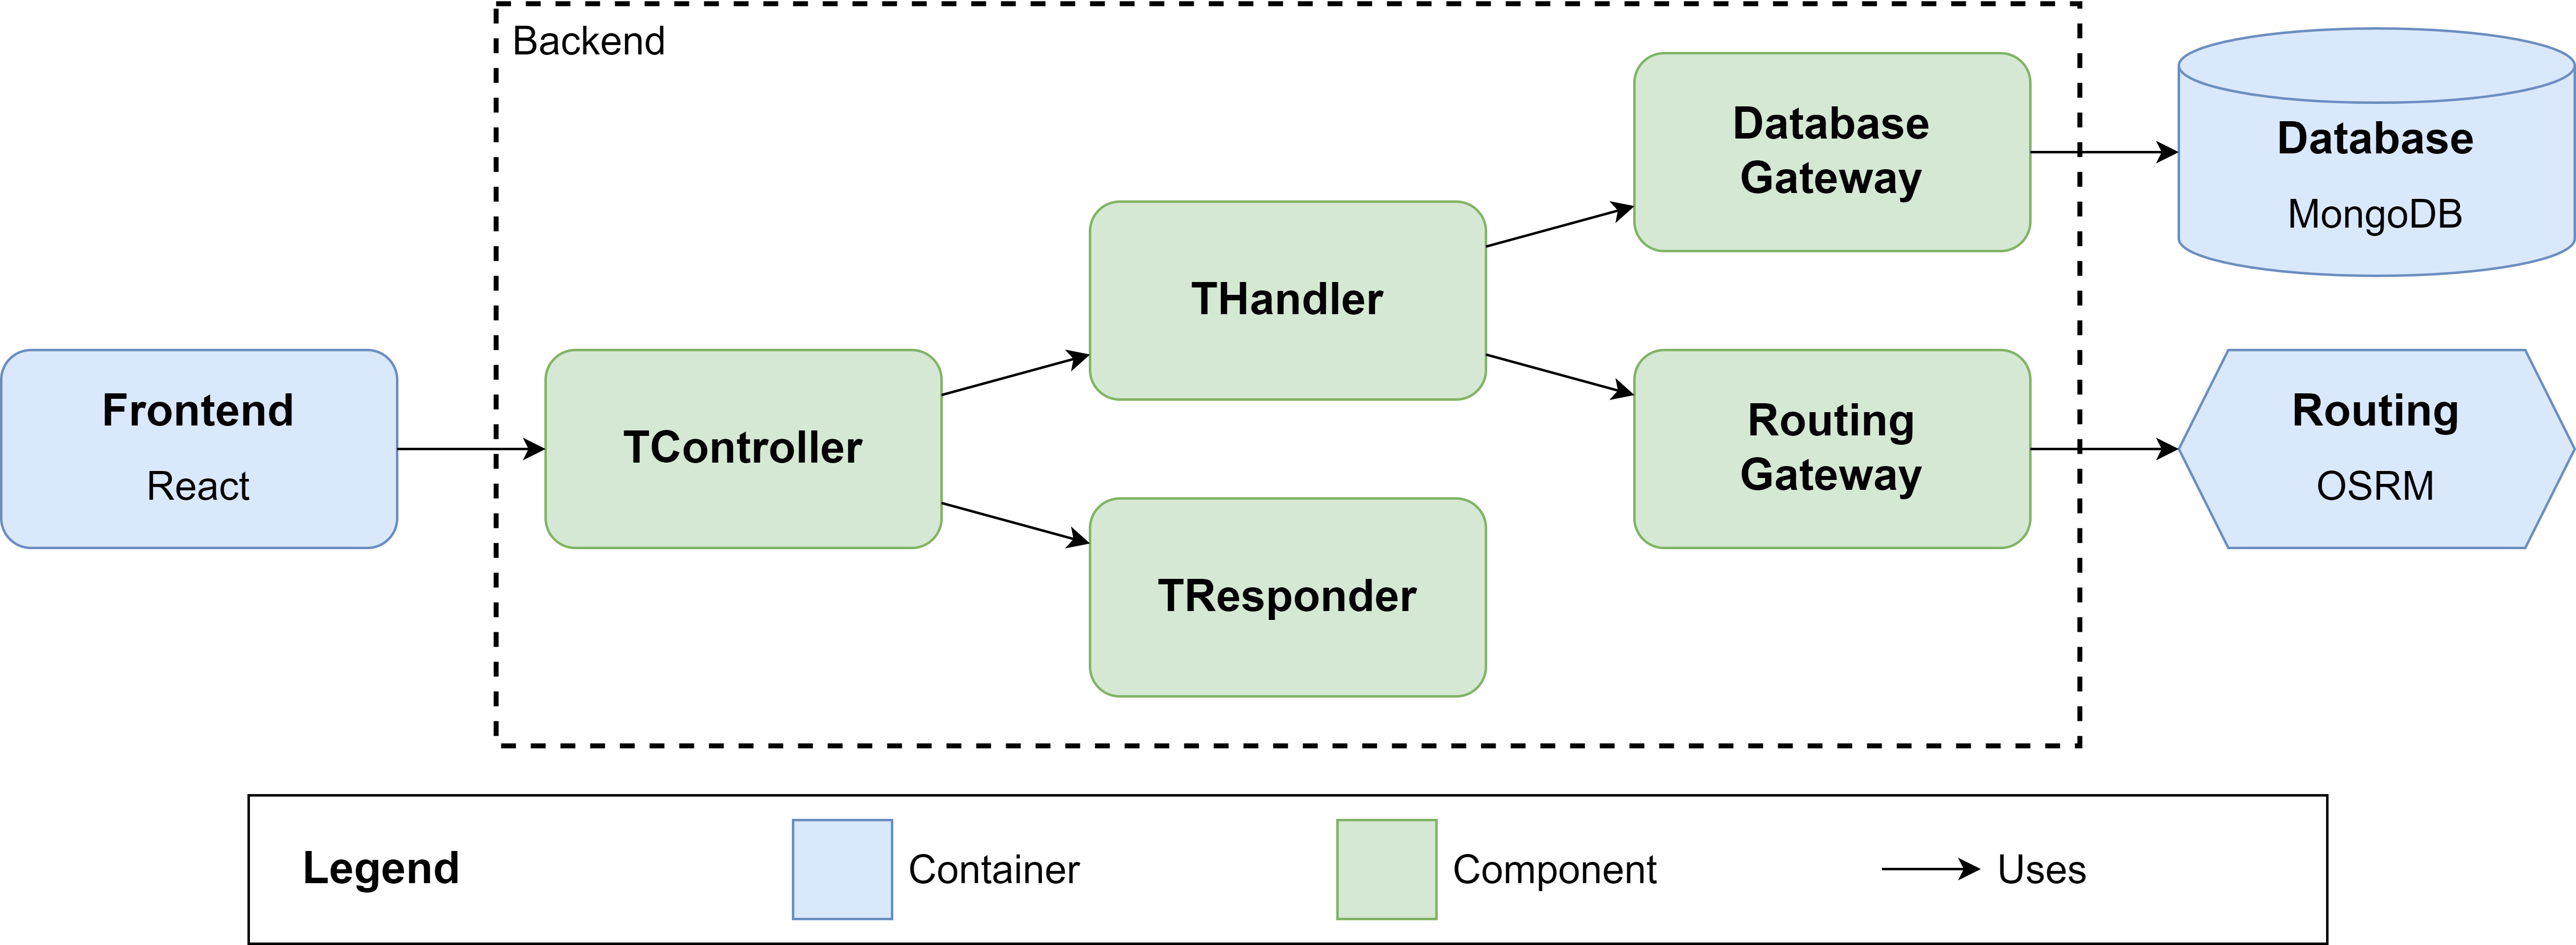
\includegraphics[width=\linewidth]{img/design/c4-component-diagram-backend.png}
\caption{C4 component diagram of the Backend container.}
\label{fig:c4-component-diagram-backend}
\end{figure}

Another design approach we apply while writing source code, which positively influences code modifiability and testability, is the Onion Architecture~\cite{palermo08}. The pattern relies on a more general \ac{dip} and places the domain model at the top of the hierarchy. In our solution, the entities defined in Section~\ref{sec:conceptual-model} and planning algorithms are positioned at the center. Use cases~are implemented with the help of specific \emph{handlers} that depend on the core primitives, and instances of infrastructural \emph{gateways} are injected into \emph{controllers}.

As in the previous section, we provide an overview of the technologies used later. Let us begin with a discussion of the programming language. The \emph{backend} is expected to perform computationally intensive tasks. Reasonable assumptions regarding its runtime include a managed environment with garbage collector, support for asynchronous operations, native multi-threading, and accessibility to other developers. The most suitable languages appeared to be Java and C\#\footnote{\href{https://learn.microsoft.com/en-us/dotnet/csharp/}{https://learn.microsoft.com/en-us/dotnet/csharp/}}, and we choosed the latter due to the author's prior experience.

The next step is to select a technology for creating the \acs{api}. The most ob\-vi\-ous approach is to implement separate endpoints over \acs{http} protocol for each query type. An advantage is that, since the \emph{backend} is essentially \emph{stateless}, calculated results could be effectively cached by the server and intermediaries. Other options,~such as GraphQL\footnote{\href{https://graphql.org/}{https://graphql.org/}}, SOAP\footnote{\href{https://www.w3.org/TR/soap12-part1/}{https://www.w3.org/TR/soap12-part1/}}, and gRPC-Web\footnote{\href{https://grpc.io/docs/platforms/web/}{https://grpc.io/docs/platforms/web/}}, were considered but deemed too advanced or atypical for our use cases.

A standard framework for building web applications in C\# is ASP.NET Core\footnote{\href{https://learn.microsoft.com/en-us/aspnet/core/?view=aspnetcore-6.0}{https://learn.microsoft.com/en-us/aspnet/core/?view=aspnetcore-6.0}}. It offers configurable request processing pipelines and out of the box dependency injection container.

There are two main approaches to creating an \acs{http} interface with ASP.NET Core: minimal and controller-based APIs\footnote{\href{https://learn.microsoft.com/en-us/aspnet/core/fundamentals/apis?view=aspnetcore-6.0}{https://learn.microsoft.com/en-us/aspnet/core/fundamentals/apis?view=aspnetcore-6.0}}. The first approach skips most of the boilerplate code; endpoints are defined in terms of lambda functions directly attached to respective routes. Despite its simplicity, minimal \acs{api} lacks support for model validation, among other things. Thus, we select the second, which~enforces design patterns and conventions for code organization.

\subsection{Database}\label{ssec:design-database}

% https://solr.apache.org/guide/solr/latest/query-guide/spatial-search.html
% https://www.elastic.co/guide/en/elasticsearch/reference/current/geo-queries.html

Data collected from various sources ends up in the \emph{database}, a container within the data tier. This segment of the architecture should ultimately behave as public storage from Section~\ref{sec:definitions} accessible through the \emph{backend}. Based on the re\-quire\-ments analysis, we have divided the capabilities into two semantically independent subsets, each designed to accomplish certain tasks.

The first group enforces the \emph{database} to act as a \emph{store}. Those include fetching places by an identifier and the ability to accommodate arbitrarily large amounts of possibly incomplete entities (the presence of keys in the \texttt{attributes} is not stable across the collection).

The second role is an \emph{index} with a focus on facilitating search queries. In~some sense, these capabilities are orthogonal to the previously mentioned ones but are equally important, as they directly affect the system's ability to fulfill Requirements~\ref{itm:q-response-time-places} and \ref{itm:q-response-time-routes}. We expect this container to be able to:

\begin{enumerate}
\item suggest the \emph{k} most relevant keywords for a given prefix,
\item find all places around some center point ordered by the crow-fly distance or within an arbitrary polygon with no distance constraints,
\item and have a mechanism to express all six types of attribute filters.
\end{enumerate}

A commonly applied practice is to implement these roles as two services: the store with entities and the index holding only the information to be queried. Together with the routing engine, this separation would make the system challenging to run on a personal computer, as the setup would require allocating substantial hardware resources. Therefore, the goal is to consolidate all func\-tion\-al\-ity into~one container without compromising performance.

We should note that a relational database with ACID properties would not be a good fit, mainly due to the unbounded size of the place collection and its heterogeneity. At the same time, spatial queries are well-supported by PostGIS\footnote{\href{https://postgis.net/}{https://postgis.net/}} extension for PostgreSQL, and the database itself is used by the \acs{osm} project.

The alternative is to consider a NoSQL database with support for spatial queries, a weak schema, and horizontal scaling. To simplify the decision-making process, we refer to the article by Guo and Onstein~\cite{guo20}, where they reviewed ten of the most popular NoSQL solutions. Taking into account their overview and the fact that places, as defined by the \emph{\nameref{sec:conceptual-model}}, exist as isolated bundles, we conclude that MongoDB\footnote{\href{https://www.mongodb.com/}{https://www.mongodb.com/}}, a document-oriented database, successfully addresses our needs.

The last observation is that keyword suggestions are likely to be the most frequent requests, primarily because place and route search queries depend on their results. Answering them without disturbing the \emph{database} is highly desirable. We assume that the collection of keywords is small enough to fit in the main memory, and such requests can be carried out by the PruningRadixTrie\footnote{\href{https://github.com/wolfgarbe/PruningRadixTrie}{https://github.com/wolfgarbe/PruningRadixTrie}}, a~high-performance data structure written in C\#.

\subsection{Routing}\label{ssec:design-routing}

According to Figures~\ref{fig:ui-result-routes} and \ref{fig:ui-result-direcs}, the application should present any route or direction to the user using points of interest and a polygonal chain drawn on the map. The segments of this chain should overlap with the actual street network~to achieve the desired level of precision. Since most of our locations come from~\acs{osm}, it is also rational to use this dataset as the basis for finding traversals.

Implementing a routing engine would have a scale infeasible for one developer. For this reason, we rely on one of the most popular open-source projects in this field. Please refer to the overview \cite{nolde20} for more details.

Due to the focus on efficiency and variety of results stated in \ref{itm:q-efficiency-variety}, we select \ac{osrm}\footnote{\href{https://project-osrm.org/}{https://project-osrm.org/}} written in optimized C++. To achieve high performance in calculations, this engine builds hierarchies of pre-computed shortcuts that enable early pruning of candidate vertices that would fail to contribute to the final result. As a tradeoff, \acs{osrm} is quite resource consuming, but we have already freed up sufficient computation power and memory by merging store and index in one container.

\subsection{Personal storage}\label{ssec:personal-storage}

As specified in Requirement~\ref{itm:q-solid-indexeddb}, both device and personal storages should be used interchangeably. In principle, only a \acs{solid} pod would be enough, but several drawbacks led us to incorporate a fallback.

\begin{itemize}
\item \acs{solid} is a promising technology with far-reaching implications concerning data ownership, and it requires an understanding of the related concepts. However, not many users are willing to invest additional effort.
\item The \acs{solid} protocol does not have a finalized version. According to the~doc\-u\-men\-ta\-tion: \emph{``This document may be updated, replaced or obsoleted by other documents at any time. It is inappropriate to cite this document as other than work in progress~\cite{solid22}.''}
\item There is currently no market-ready \acs{solid} implementations or providers with guaranteed quality of service.
\end{itemize}

In this thesis, we target only Inrupt PodSpaces\footnote{\href{https://docs.inrupt.com/pod-spaces/}{https://docs.inrupt.com/pod-spaces/}} with instances of \ac{ess}\footnote{\href{https://docs.inrupt.com/ess/latest/}{https://docs.inrupt.com/ess/latest/}}. We use Inrupt JavaScript Client Libraries\footnote{\href{https://docs.inrupt.com/developer-tools/javascript/client-libraries/}{https://docs.inrupt.com/developer-tools/javascript/client-libraries/}} to authenticate against servers and perform data access operations. The frontend has also been tested on Community\footnote{\href{https://github.com/CommunitySolidServer/}{https://github.com/CommunitySolidServer/}} and Node\footnote{\href{https://github.com/nodeSolidServer/}{https://github.com/nodeSolidServer/}} Solid Servers, yielding positive outcomes.

\acs{solid} allows for storing both structured and unstructured data. The former would be advantageous if we were to expose this information to other agents, but this is not the case. As a simplification, it is assumed that entities are saved as separate \acs{json} files in the \emph{hardcoded} folder \texttt{\$\{storage-root\}/smartwalk/}.

\subsection{Tile provider}\label{ssec:tile-provider}

Results of queries are presented on the map together with square-shaped tiles, visually representing the corresponding local area. Tiles are typically distributed in two forms: raster pictures rendered on the server side and vector graphics~ren\-dered by a client. As smartphones are among the supported platforms, pictures fit better due to their optimized power consumption pattern.

We use \acs{osm} standard tile provider. It is permitted\footnote{\href{https://operations.osmfoundation.org/policies/tiles/\#requirements}{https://operations.osmfoundation.org/policies/tiles/\#requirements}} as long as the application does not generate too much traffic. Tiles are downloaded using the following link, where \texttt{s} stands for a subdomain (optional parameter), \texttt{x} and \texttt{y} point to a rectangle in the grid, and \texttt{z} is a zoom level:

\begin{center}
\texttt{https://\$\{s\}.tile.openstreetmap.org/\$\{z\}/\$\{x\}/\$\{y\}.png}.
\end{center}

\section{Data preparation}\label{sec:data-preparation}

% https://www.mongodb.com/docs/manual/geospatial-queries/
% https://www.mongodb.com/docs/manual/reference/glossary/#std-term-WGS84

Potential data sources and distribution methods were discussed in Section~\ref{sec:data-sources}, but not all of them were equally good for our needs. We utilize only the following \emph{five} distributions in the prescribed way.

\acs{osm} dump files, published in PBF format, are used to build graph structures for \acs{osrm} and populate the database. The first procedure is done automatically by standard tools, with details given in Attachment~\ref{sec:documentation}, Administrator's guide. The other part is our responsibility.

PBF files can be handled as a stream of elements using the OsmSharp\footnote{\href{http://www.osmsharp.com/}{http://www.osmsharp.com/}} library written in C\#. Unfortunately, the \acs{osm} data model does not restrict the shape~of tags. Hence, we need to implement custom parsers.

The community recognized this problem and established naming conventions and guidelines. Taginfo helps to identify the most popular keys and \emph{frequencies}~of values associated with them. This information allows us to filter out infrequent strings by setting a threshold and develop finer-grained extractors. The service~ex\-pos\-es an \acs{http} endpoint so that the statistics for a given key can be retrieved~via a simple \texttt{GET} request.

Determining a location for \emph{relation}-type \acs{osm} elements is not straightforward. We must retain all references to nodes and ways with coordinates in the main memory, and the task becomes too large to accomplish on an ordinary computer. Instead, these smaller requests are delegated to Overpass~API.~The~service precomputes the \emph{centers} of multi-polygonal bodies, which we retrieve in bulk using the following query sent in the \texttt{data} parameter of an \acs{http} \texttt{GET} request:

\begin{minted}{text}
/* s, w, n, e should form a valid bounding box */
[out:json];
relation(${s},${w},${n},${e})[type=multipolygon];
out center;
\end{minted}

We mentioned earlier that Wikidata has a predictable internal structure and can be considered an independent source of geographic data. In contrast, triples in DBPedia are inherently more abstract. Hence, it makes sense to separate the process of ingesting data from knowledge graphs into two self-contained steps: creating simple stubs with georeferences from Wikidata that do not yet exist and enriching (or updating) places.

To obtain locations, we utilize a slightly modified version of the query mentioned in Section~\ref{ssec:wikidata}. In particular, matching by the property~path \texttt{P31/P279*} is a time-consuming operation and should be omitted.

The following query serves a generic template to handle the \emph{enrichment} step.

\begin{minted}{text}
PREFIX my: <http://www.example.com/#>
PREFIX owl: <http://www.w3.org/2002/07/owl#>

CONSTRUCT {
  ?wikidataId
    my:dbpedia ?dbpediaId;
    my:param ?param.
}
WHERE {
  VALUES ?wikidataId {
    ${l} # expand a list of Wikidata identifiers
  }
  ?dbpediaId owl:sameAs ?wikidataId.
  OPTIONAL {
    ?dbpediaId ${p} ?param. # replace by a predicate
  }
  ... more OPTIONAL blocks follow ...
}
\end{minted}

The result of this query is a new \acs{rdf} graph due to the \texttt{CONSTRUCT} clause. To narrow the search and focus solely on relevant entities, the \texttt{VALUES} block~pre\-scribes possible values that the \texttt{wikidataId} variable can hold. This block is~pop\-u\-lat\-ed with Wikidata identifiers available in our database. Some targeted properties might be missing, and we should consider partial matches as valid results. The \texttt{OPTIONAL} block encloses optional parts of the graph pattern. Furthermore, the predicate \texttt{owl:sameAs} establishes an equality relation between entities from different knowledge graphs.

Wikidata and DBPedia are queried via \acs{http} endpoints that accept percent-encoded \acs{sparql} queries in the \texttt{query} parameter. To simplify response handling, we employ content negotiation in the way described below.

\begin{enumerate}
\item Request data with the \texttt{Accept} header set to \texttt{application/n-triples} for DBPedia and \texttt{application/n-quads} for Wikidata.
\item Parse response string into \acs{jsonld}, and compact the graph using injected \texttt{@context}. This step is carried out by the jsonld\footnote{\href{https://www.npmjs.com/package/jsonld}{https://www.npmjs.com/package/jsonld}} library.
\item We receive a plain JavaScript object with the known property configuration as the output.
\end{enumerate}

Eventually, a place could have up to \emph{40} distinct attributes. Some of these attributes are aggregated into larger objects, resulting in only \emph{29} that are queryable.

Below, we note two more rules that should be followed to ensure the feasibility of data preparation procedures and the correctness of the input.

\begin{itemize}
\item Routines extracting or fetching places have a \emph{bounding box} as a compulsory input parameter.
\item As a matter of fact, MongoDB uses coordinates given in the \emph{WGS84} \ac{crs} to index spatial objects. Fortunately, all~the in\-for\-ma\-tion repositories we consider comply with that \acs{crs}. Otherwise, location references would need to be translated before writing to the database.
\end{itemize}

\section{Routing algorithms}\label{sec:routing-algorithms}

The final piece of information we need before moving to the next chapter~is how to map the route search defined by Requirements~\ref{itm:f-search-routes-automatic} to \ref{itm:f-search-routes-valid} onto a theoretical framework. A better understanding of the underlying mathematics positively affects our reasoning abilities and later implementation.

First, various formalizations are described, culminating in one that best aligns with our needs. Subsequently, two polynomial-time heuristics are presented, capable of finding ``valid'' routes from \ref{itm:f-search-routes-valid}.

We expect thorough knowledge of the basic courses on discrete mathematics and theory of computation, typically covered in a standard Computer Science~curriculum. Please refer to~\cite{matousek08,diestel17,sipser13} for a refresher, or feel free to skip this section if theoretical aspects are not of interest to you.

\subsection{Notation}\label{ssec:notation}

Imagine a map of some city as a collection of objects, where business centers, pharmacies, and shops are interconnected by sidewalks, highways, and roads. A \emph{finite graph} is an abstract model that accurately describes structures of this kind. To avoid misunderstanding, we provide formal definitions of concepts used in this section; most of them can be found in the literature referred to just above.

A \emph{graph} $G$ is an ordered pair $(V, E)$, where $V$ is a set of \emph{vertices} (points drawn on the map), and $E$ is a set of \emph{edges} (roads and sidewalks). We do not consider multigraphs, and thus, $E \subseteq V^{2}$. $\left| V \right|$ is the \emph{order} of a graph, and $\left| E \right|$ is its \emph{size}. If all edges of a graph satisfy the property $(u, v) \in E \Leftrightarrow (v, u) \in E$, the graph is said to be \emph{undirected} and \emph{directed} otherwise. \emph{Complete} graphs are those having all possible edges, that is, $E = V^{2}$.

A \emph{walk} is an alternating sequence of vertices and edges $(v_{0}, e_{1}, v_{1}, \ldots, v_{n})$, such that $v_{i} \in V$ and $e_{i} = (v_{i}, v_{i+1}) \in E$. A \emph{trail} is a walk with distinct edges. A~\emph{path} is a walk with distinct vertices. A \emph{Hamiltonian path} is a path containing all~vertices of a graph. Similarly, a \emph{closed walk}, \emph{closed trail}, \emph{cycle}, and \emph{Hamiltonian cycle} are defined by setting $v_{0} = v_{n}$. We occasionally use $s$ to denote a starting vertex and $t$ to represent a target.

Distances between vertices are determined by a non-negative \emph{distance function} $d: E \to \mathbb{R}_{\geq 0}$. The total distance of a (closed) walk is calculated as the sum~of the dis\-tances of all visited edges and, if necessary, is bounded above by $D_{\text{max}}$.

Please recall the function $m : V \times C \to \{ 0, 1 \}$ for categorical matching introduced in Section~\ref{sec:definitions}; its definition remains the same. The exis\-tence of an arrow between any two categories is given by an \emph{arrow function} $a: C^{2} \to \{ 0, 1 \}$ whose value $a(c_{1}, c_{2}) = 1$ if a place matched by $c_{1}$ must precede another place matched by $c_{2}$ on a path, and $0$ if this is not the case.

\subsection{Formalization}\label{ssec:formalization}

The goal is to gradually generalize problem statements until we find a suitable one. Figure~\ref{fig:overview-npo-problems} summarizes our endeavor. Let us start with the definition of~a particular \emph{decision problem}; a proof of its NP-completeness can be found in~\cite{karp72}.

\begin{definition}[HamCycle]
Does a graph $G$ have a Hamiltonian cycle?
\end{definition}

Even though this problem is NP-complete, and the existence of an efficient algorithm solving it is unlikely, there is no way to express the distance of a cycle, among other limitations. Therefore, we propose the following extension: the~well-known \ac{tsp}.

\begin{definition}[\acs{tsp}]\label{def:tsp}
How long is the shortest Hamiltonian cycle in a complete graph $G$ with a distance function $d$?
\end{definition}

A careful reader might argue that there is a decision variant of the \acs{tsp}. One interesting aspect of Definition~\ref{def:tsp} is that it seeks the shortest cycle, representing the best possible or optimal solution for the given settings. Moreover, the HamCycle is reducible to the \acs{tsp} by setting values of the distance function to $1$ for~all $e \in E$, and $2$ otherwise. Then, we ask whether the shortest Hamiltonian cycle in $G$ has the length of $\left| V \right|$. This shows the NP-hardness of the \acs{tsp}.

All route search formalizations targeted in this thesis, including the \acs{tsp},~are \emph{NP-optimization problems} defined over possibly large but finite graphs. In principle, we could solve them by enumerating all configurations. Unfortunately, this idea becomes impractical for sufficiently large instances. In the \acs{tsp}, the number of cycles grows factorially with the order of $G$.

Considering the current state of knowledge, we cannot hope to obtain an~optimal solution in a reasonable time, even for the simplest problems, leaving aside categories and arrows. Sometimes, a \emph{near-optimal} solution is enough if computed efficiently.

\begin{definition}[$\alpha$-approximation algorithm~\cite{williamson10}]
An \emph{$\alpha$-approximation algorithm} for an NP-optimization problem is a polynomial-time algorithm that for all instances of the problem produces a solution whose value is within a factor of $\alpha$ of the value of an optimal solution.
\end{definition}

Sahni and Gonzalez~\cite{sahni76} showed that an $\alpha$-approximation for the \acs{tsp}, with~no further restrictions on the distance function, implies the solvability of the HamCycle in polynomial time. The existence of such an algorithm is unlikely.

The reason HamCycle could be solved is that the distance function does not always respect the triangle inequality $\forall u, v, w \in V : d(u, w) \leq d(u, v) + d(v, w)$. To\-geth\-er with this inequality, $d$ becomes a \emph{quasimetric}. In practice, one might en\-counter two cases of the \acs{tsp} equipped with such a function: the \ac{atsp} and the \ac{stsp}.

The asymmetric alternative covers everyday needs better because transportation networks typically disregard symmetry. However, this generalization appears particularly difficult to deal with. Only recently, Traub and Vygen~\cite{traub20} designed a highly non-trivial $(22+\varepsilon)$-approximation algorithm based on the results of many other researchers.

Fortunately, \acs{stsp} is approximable by polynomial-time heuristics with a much better constant ratio. Christofides~\cite{christofides76} employed a composition of minimum spanning tree and minimum-weight perfect matching to devise a $3/2$-approximation. Since then, only subtle progress has been made towards achieving a lower factor.

Till now, we have been discussing the \acs{tsp} that aims to obtain a Hamiltonian cycle, but certainly, finding a \emph{path} would reflect Requirement~\ref{itm:f-search-routes-valid} better. Again, the best approximation algorithms achieve ratios of $43 + \varepsilon$ for the \acs{atsp} due to Traub and Vygen~\cite{traub20} and $3/2$ for the \acs{stsp} due to Zenklusen~\cite{zenklusen18}.

Taking into account the fundamental difficulty of the \acs{atsp}, we conclude that the \acs{stsp} is the most appropriate formalization to consider when selecting or de\-sign\-ing more capable algorithms. This was also one of the reasons we support only the walking mode, since sidewalks are assumed to be passable in both directions, ensuring that the distance function of a problem instance is symmetric.

In the remainder, we discuss more relevant problem statements without details on known approximation ratios. Instead, we leave pointers for further exploration.

\vspace{0.5em}

Let us proceed with an extension of the \acs{tsp}, the \ac{op}. Its input also includes a starting point $s$ and destination $t$, non-negative function $score: V \to \mathbb{R}_{\geq 0}$, and upper bound $D_{\text{max}}$. An instance of the \acs{op} seeks for~a~path from $s$ to $t$ with a length no longer than $D_{\text{max}}$ that visits a subset of $V$, maximizing the total collected score~\cite{gunawan16}.

Although we have addressed the distance, it is not clear how to map a category to the set of real numbers. The \emph{\nameref{ssec:city-trip-planner}} used a variant of the \acs{op}, the \ac{ttdp}, and accomplished this task by converting user input into the sum of type, category, and keyword search scores~\cite{vansteenwegen11}.

\vspace{0.5em}

The \acs{op} enables us to reason about places in terms of \emph{relevancy}, but our cat\-e\-gories match them \emph{precisely}. The \ac{gtsp} offers a toolset that captures the discrete nature of keywords and attribute filters.

\begin{definition}[\acs{gtsp}~\cite{pop23}]
Given a complete graph $G$ whose vertices are divided into a given number of mutually exclusive clusters, denoted by $L_{1}, L_{2}, \ldots, L_{k}$, and a distance function $d$, the GTSP searches for the shortest cycle visiting a~collection of vertices with the property that at least one vertex from each cluster is visited.
\end{definition}

Li et al.~\cite{li05} proposed the \ac{tpq}, a path version of the \acs{gtsp} with a symmetric distance function. Cao et al.~\cite{cao12} studied approximation algorithms and heuristics for the \ac{kor}, a modification of the \acs{gtsp} in which the total distance is bounded above. In~both \acs{tpq} and \acs{kor}, clusters are expressed by means of distinct keywords.

It is worth mentioning that our places could satisfy more than one category~at once; a simple reduction to an instance of the \acs{gtsp} is to define $V$ as a set of~tuples $(\text{place}, \text{category})$.

Finally, we need to provide users with a way to \emph{order} clusters. The~\ac{pcgtsp}~\cite{pop23} incorporates arrows and enforces specific arrangements using directed acyclic graphs. Similar to the \acs{gtsp}, there are less abstract interpretations of the same problem focused on real-world applications. In particular, the \ac{mrpsr}~\cite{chen08} and \ac{osr}~\cite{sharifzadeh08} cover \emph{partial} and \emph{linear} orders, respectively.

\vspace{0.5em}

In this thesis, we consider the \acs{gtsp} and \acs{pcgtsp} as baseline formalizations for unordered and ordered instances, respectively, around which all algorithms and heuristics should evolve. Both lack a mechanism for limiting the distance~of a path. As we will see in Section~\ref{ssec:finding-a-sequence}, calculating a \emph{network distance} is a~time and resource consuming process, leading us to opt for estimation. Hence, sat\-is\-fy\-ing this constraint at all costs becomes meaningless.

\begin{figure}[!h]
\centering
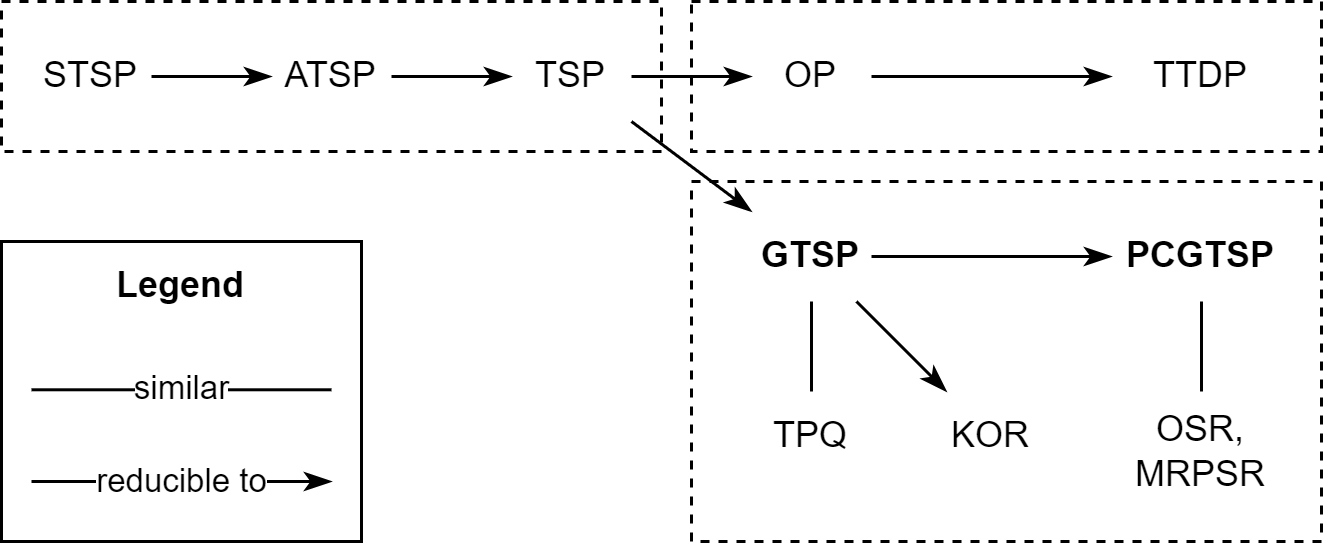
\includegraphics[width=0.9\linewidth]{img/design/overview-npo-problems.png}
\caption{An overview of the related NP-optimization problems.}
\label{fig:overview-npo-problems}
\end{figure}

\subsection{Finding a sequence}\label{ssec:finding-a-sequence}

Two polynomial-time heuristics \emph{without} performance guarantees are described at the beginning of this section, one for the \acs{gtsp} and another for the \acs{pcgtsp}. Relaxed requirements on optimality are aligned with \ref{itm:q-efficiency-variety}. Finally, the geometric jus\-ti\-fi\-ca\-tion of the place retrieval process is given, and two realizations of a dis\-tance function are considered.

\subsubsection*{Unordered categories}

To solve unconstrained instances, we utilized \ac{ifh} designed by Kanza et al.~\cite{kanza08}. This iterative procedure unfolds as follows.

\begin{algorithm}
\caption{\acl{ifh}.}\label{alg:if-heuristic}
\begin{algorithmic}
\Function{IfHeuristic}{$V, C = \{ c_{1}, \ldots, c_{k} \}, m, d, s, t$}
  \State $\mathcal{S} \gets \left[ s, t \right]$ \Comment{Initialize a sequence}
  \For{$c_{i} \in C$}
    \State $M_{i} \leftarrow \{ v : v \in V \wedge m(v, c_{i}) = 1 \}$ \Comment{Find matching places}
  \EndFor
  \State $\mathcal{M} \gets \left[ M_{1}, \ldots, M_{k} \right]$ sorted by cardinality in ascending order
  \ForAll{$M$ of $\mathcal{M}$ in a given order}
    \State $v, i \gets \textsc{SelectBest}(\mathcal{S}, M, d)$
    \State $\mathcal{S} \gets \textsc{InsertAt}(\mathcal{S}, v, i)$
  \EndFor
  \State \Return $\mathcal{S}$
\EndFunction
\end{algorithmic}
\end{algorithm}

The \textsc{SelectBest} determines a place in the given set $M$ and an index within the current sequence $\mathcal{S}$ that, if inserted, minimizes the impact on the length. The selection criterion is illustrated in Figure~\ref{fig:if-heuristic}, where the blue dot is the candidate place, two blue edges with ``+'' contribute to the total distance, and the one with ``--'' is removed from the configuration.

\begin{figure}[!h]
\centering
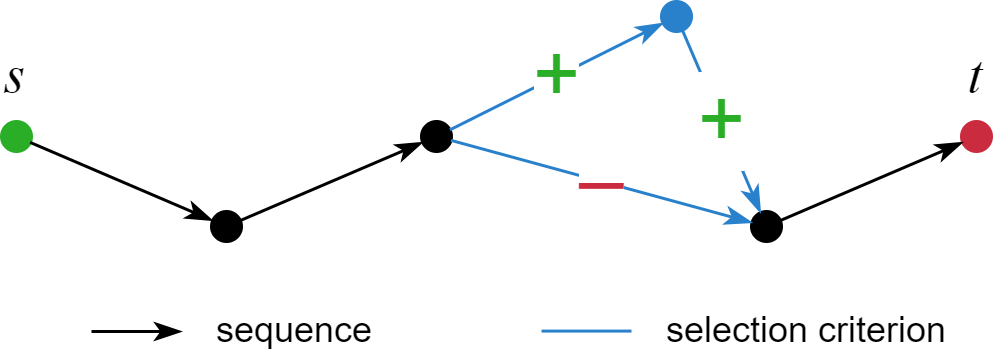
\includegraphics[width=0.65\linewidth]{img/design/if-heuristic.png}
\caption{Infrequent-First Heuristic, selection criterion.}
\label{fig:if-heuristic}
\end{figure}

The time complexity of this algorithm is dominated by the \textbf{for}-cycle over $\mathcal{M}$ resulting in $O(\lvert V \rvert \lvert C \rvert^{2})$.

% \begin{equation*}
% O(\lvert V \rvert \lvert C \rvert + \lvert C \rvert \log \lvert C \rvert + \left( \lvert V \rvert \lvert C \rvert + \lvert C \rvert \right) \cdot \lvert C \rvert)
% \end{equation*}

After finding a feasible route, we could try to improve the sequence via local search. One of the most popular and simple heuristics is called $2$-Opt. For every pair of edges, $\{ u_{1}, v_{1} \}$ and $\{ u_{2}, v_{2} \}$, we redefine them as $\{ u_{1}, u_{2} \}$ and $\{ v_{1}, v_{2} \}$ and accept change if the total length decreases. The procedure is repeated as long as such a pair exists.

Even though $2$-Opt has a very concise description, there are graphs proposed by Englert, R\"{o}glin, and V\"{o}cking~\cite{englert14} on which it can make an exponential number of steps. Despite this, we include it as a subroutine because our paths~are typically short.

\subsubsection*{Ordered categories}

Kanza et al.~\cite{kanza10} developed the \ac{ogh} to address precedence constraints, the implementation details are shown in Algorithm~\ref{alg:og-heuristic}.

\begin{algorithm}
\caption{\acl{ogh}.}\label{alg:og-heuristic}
\begin{algorithmic}
\Function{OgHeuristic}{$V, C = \{ c_{1}, \ldots, c_{k} \}, m, d, a, s, t$}
  \State $\mathcal{S} \gets \left[ s, t \right]$ \Comment{Initialize a sequence}
  \For{$c_{i} \in C$}
    \State $M_{i} \leftarrow \{ (v, i) : v \in V \wedge m(v, c_{i}) = 1 \}$ \Comment{Find matching tuples}
  \EndFor
  \State $\mathcal{M} \gets \left\{ M_{1}, \ldots, M_{k} \right\}$
  \While{$\mathcal{M} \neq \emptyset$}
    \State $U \gets \bigcup \{ M_{i} : M_{i} \in \mathcal{M} \wedge \left( \not\exists M_{j} \in \mathcal{M} : a(c_{j}, c_{i}) = 1 \right) \}$ \Comment{Find candidates}
    \State $(v, i^{\prime}) \gets \textsc{SelectBest}(\mathcal{S}, U, d)$
    \State $\mathcal{M} \gets \mathcal{M} \setminus \{ M_{i^{\prime}} \}$
    \State $\mathcal{S} \gets \textsc{InsertAt}(\mathcal{S}, v, \lvert \mathcal{S} \rvert)$
  \EndWhile
  \State \Return $\mathcal{S}$
\EndFunction
\end{algorithmic}
\end{algorithm}

The semantics of the \textsc{SelectBest} here are slightly different than that of~the corresponding function in \acs{ifh}, as illustrated in Figure~\ref{fig:og-heuristic}. The candidate vertex is always inserted between $t$ and the one just before it. Furthermore, only the blue $(+)$-edges participate in decision-making. The criterion, defined as the sum of the distances, ensures that places are selected as close to the straight line connecting $s$ and $t$ as possible and that the sequence does not progress too fast towards the target. The blue edges with arrow tips are added to the final configuration, and the black one marked ``$\times$'' is removed.

\begin{figure}[!h]
\centering
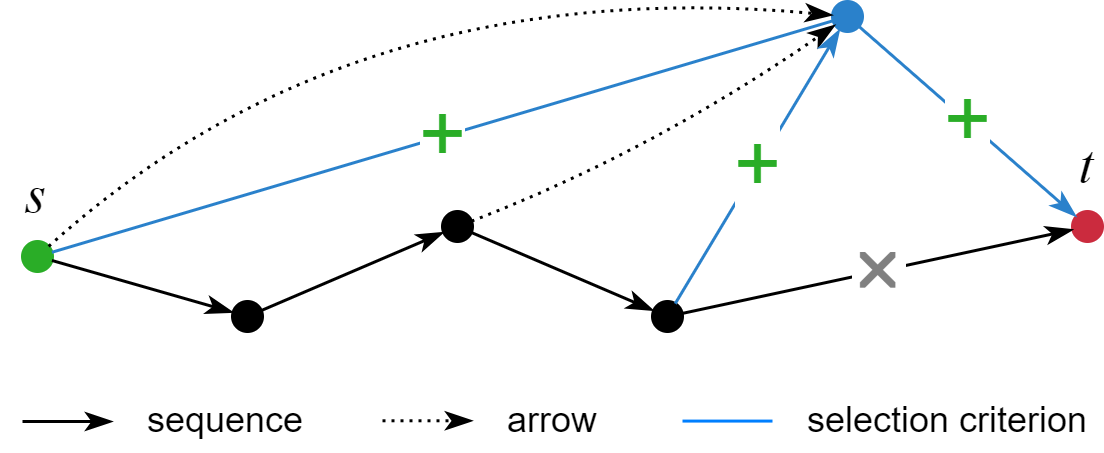
\includegraphics[width=0.70\linewidth]{img/design/og-heuristic.png}
\caption{\acl{ogh}, selection criterion.}
\label{fig:og-heuristic}
\end{figure}

Since each $M_{i}$ can contain at most $\lvert V \rvert$ tuples, an iteration of the \textbf{while}-cycle has a time complexity of $O(\lvert V \rvert \lvert C \rvert)$. Therefore, this heuristic runs in $O(\lvert V \rvert \lvert C \rvert^{2})$, which is as fast as \acs{ifh}.

% \begin{equation*}
% O(\lvert V \rvert \lvert C \rvert + \left(\lvert V \rvert \lvert C \rvert + \lvert V \rvert \lvert C \rvert + \lvert C \rvert + 1 \right) \cdot \lvert C \rvert)
% \end{equation*}

\subsubsection*{Bounding shape}

% https://stackoverflow.com/questions/38302476/how-does-atan-appear-in-haversine-formula

The next aspect directly affecting the search speed is the cardinality of $V$.~We should agree that places lying too far from $s$ or $t$ are of little interest to us due to an upper bound on the length of a path and should be eliminated before entering an algorithm. However, it is not entirely clear how to measure distances.

First, we need an abstract geometric shape to model the surface of the Earth. The WGS84\footnote{\href{https://epsg.io/4326}{https://epsg.io/4326}: WGS84 -- World Geodetic System 1984, used in GPS} \emph{geographic} coordinate system uses an \emph{oblate spheroid}, as specified in the EPSG public registry. Calculations on an ellipsoidal body achieve~higher precision but are more computationally demanding. As a result, most web maps, in\-clud\-ing \acs{osm}, have adopted the Web Mercator\footnote{\href{https://epsg.io/3857}{https://epsg.io/3857}: WGS84 / Pseudo-Mercator -- Spherical Mercator} as a baseline \emph{projected} coordinate system for translating WGS84 points into two-dimensional space, assuming they are drawn on a \emph{sphere}. Thus, we make a similar assumption.

Once the geometry is known, a straight line distance between two given points, denoted by $d_{H}$, can be expressed using the \emph{Haversine formula}. As an alternative, we could also query the \acs{osrm} to determine a network distance $d_{N}$. Clearly, the relation $d_{H} \leq d_{N}$ holds for all pairs of vertices.

In order to filter out points lying too far from $s$ or $t$ and eventually reduce~$\lvert V \rvert$, we should retrieve only those within some \emph{bounding shape}. The most appropriate approach is to utilize the mathematical properties of an \emph{ellipse}. We set~foci $F_{1}$ and $F_{2}$, major axis $a$, and focal distance $c$ as follows, provided that $d_{H}(s, t) < D_{\text{max}}$:

\begin{equation*}
F_{1} = s, \qquad
  F_{2} = t, \qquad
    a = \frac{D_{\text{max}}}{2}, \qquad
      c = \frac{d_{H}(s, t)}{2}.
\end{equation*}

As $d_{H}(s, v) + d_{H}(v, t) \leq D_{\text{max}}$ holds for any $v \in V$ inside the ellipse or on~the bound\-ary, we may safely skip points outside, especially if final distances are de\-ter\-mined by $d_{N}$.

Our use cases assume that a starting point and destination need not lie on a horizontal line, and a basic ellipse almost always requires rotation and translation. The major obstacle related to drawing figures on a sphere is that its \emph{parallels} have different lengths. The following subroutine handles transformation properly.

\begin{enumerate}
\item Calculate the coordinates of the midpoint $o$ between $s$ and $t$ (in \emph{degrees}).
\item Define an ellipse $e$ with its center at the origin $(0, 0)$, $F_{1}$ at $(-c, 0)$, and $F_{2}$ at $(c, 0)$, where $c$ is measured in \emph{meters}.
\item Approximate $e$ by a polygon $p$ whose points lie precisely on the boundary.
\item Rotate $p$ about the origin so that it has the same orientation as the straight line connecting actual $s$ and $t$.
\item Transform $x$- and $y$-components of points of $p$ to \emph{degrees} with respect to~the parallel at the latitude of $o$, which defines the cost of one radian along the $x$-axis. The cost of a radian along the $y$-axis remains constant.
\item Translate $p$ so that its center coincides with $o$.
\end{enumerate}

\newpage

Please note that this is only an approximation that works well on small scales. An example of a rotated and translated ellipse is presented in Figure~\ref{fig:rotated-ellipse}.

\begin{figure}[!h]
\centering
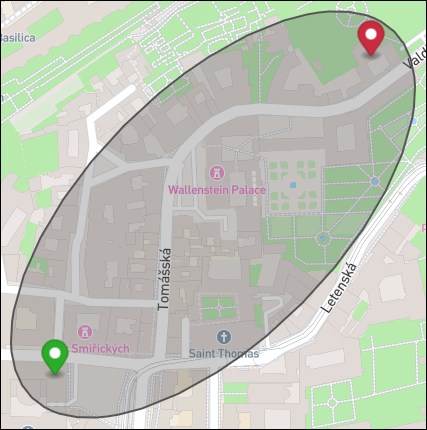
\includegraphics[width=0.5\linewidth]{img/design/rotated-ellipse.png}
\caption{Geojson.io: rotated and translated ellipse drawn on the map.}
\label{fig:rotated-ellipse}
\end{figure}

\subsubsection*{Distance function}

If we carefully review the bodies of the aforementioned heuristics, neither \acs{ifh} nor \acs{ogh} explicitly bounds the total distance of a constructed sequence.~This be\-hav\-ior is intentional, and the reason is that obtaining the length of the shortest path between two arbitrary points is a costly operation.

The \acs{osrm} has \texttt{route} and \texttt{table} services suitable for our needs. The former focuses on finding a full representation of the shortest path for a given sequence~of points, while the latter performs bulk distance calculations and can be used to~fulfill the second step in the following scenario.

\begin{enumerate}
\item Fetch the $\lvert V \rvert$ most \emph{relevant} places within a bounding ellipse.
\item Request an $\mathbb{R}^{\lvert V \rvert \times \lvert V \rvert}$ matrix containing distances between all pairs of places.
\item Use this matrix as a distance function, $d = d_{N}$.
\end{enumerate}

Recall that category matching is a boolean-valued function, implying that places cannot be sorted by relevancy. If we were to accept all matches, large values of~$\lvert V \rvert$ would inevitably increase CPU usage and memory consumption.

The only viable option, which does not require additional effort regarding~data preparation, is to set $d = d_{H}$, let an algorithm construct \emph{any} sequence preserving arrows, find the shortest path for this sequence using the \texttt{route} service, and discard those with distances larger than $D_{\text{max}}$.
